%\documentclass[11pt,letterpaper]{article}
\documentclass[acmsmall]{acmart}
% 加载 geometry 包并设置页面尺寸
%\usepackage[paperwidth=6.75in, paperheight=10in, margin=1in]{geometry}

\usepackage{stfloats}

%set page size
%\pdfpagewidth=6.75in
%\pdfpageheight=10in

%\usepackage[margin=1in]{geometry}
%\usepackage{cite}
\usepackage{hyperref}
\usepackage{colortbl}
\usepackage{paralist}
\usepackage{pdfpages}
\usepackage{enumitem}
\usepackage{float}
\usepackage{booktabs}
\usepackage[override]{cmtt}
\usepackage{color,xcolor}
\usepackage{graphicx,eso-pic}
\usepackage{boxedminipage}
\usepackage{url}
\usepackage{float}
\usepackage{caption}
\usepackage{subcaption}
\usepackage{xspace}
\usepackage{multirow}
\usepackage{amsmath,amsthm,amstext,amsfonts,latexsym}
%\usepackage{amssymb}
\usepackage{wrapfig}
\usepackage[linesnumbered,ruled,vlined]{algorithm2e}
%\usepackage{algorithm}
\usepackage[noend]{algpseudocode}
\usepackage{algorithmicx}
\usepackage{epstopdf}
\usepackage{mdframed}
\usepackage{cases}
\usepackage{mathrsfs}
\usepackage[capitalize]{cleveref}
\usepackage[compact]{titlesec}
\usepackage{tikz}
\usepackage{graphicx}
\usepackage{color}
\usetikzlibrary{positioning, shapes.geometric}
\usetikzlibrary{positioning,chains,fit,shapes,calc}

\usepackage{diagbox}



%%
%% \BibTeX command to typeset BibTeX logo in the docs
\AtBeginDocument{%
	\providecommand\BibTeX{{%
			Bib\TeX}}}

%% Rights management information.  This information is sent to you
%% when you complete the rights form.  These commands have SAMPLE
%% values in them; it is your responsibility as an author to replace
%% the commands and values with those provided to you when you
%% complete the rights form.
%\setcopyright{acmlicensed}
%\copyrightyear{2018}
%\acmYear{2018}
%\acmDOI{XXXXXXX.XXXXXXX}

%\setcopyright{acmcopyright}
% See completed rightsreview form for your code
%\acmJournal{PACMMOD}
%\acmYear{2025} \acmVolume{3} \acmNumber{3 (SIGMOD)}
%\acmArticle{161} \acmMonth{6} \acmPrice{}
% XXX is your article id# (for example: V3mod122 = your article # is 122)
%\acmDOI{10.1145/XXXXXXX}

%% These commands are for a PROCEEDINGS abstract or paper.
%\acmConference[Conference acronym 'XX]{Make sure to enter the correctconference title from your rights confirmation emai}{June 03--05, 2018}{Woodstock, NY}
%%
%%  Uncomment \acmBooktitle if the title of the proceedings is different
%%  from ``Proceedings of ...''!
%%
%%\acmBooktitle{Woodstock '18: ACM Symposium on Neural Gaze Detection,
	%%  June 03--05, 2018, Woodstock, NY}
%\textcolor{red}{comment this?}

%\acmISBN{978-1-4503-XXXX-X/18/06}
\setcopyright{acmlicensed}
\acmJournal{PACMMOD}
\acmYear{2025} \acmVolume{3} \acmNumber{3 (SIGMOD)} \acmArticle{161} \acmMonth{6}\acmDOI{10.1145/3725405}




\title{Faster and Efficient Density Decomposition via Proportional Response with Exponential Momentum}


%\author{T-H. Hubert Chan\thanks{Department of Computer Science, the University of Hong Kong.} \and Quan Xue\samethanks}
%\author{T-H. Hubert Chan}{Department of Computer Science, University of Hong Kong}{hubert@cs.hku.hk}{https://orcid.org/0000-0002-8340-235X}{This research was partially supported by the 
	%Hong Kong RGC grants 17201823, 17203122 and 17202121.}

%\author{Quan Xue}{Department of Computer Science, University of Hong Kong}{csxuequan@connect.hku.hk}{https://orcid.org/0009-0001-5939-7271}{}
%\author{Quan Xue}
%\date{July 2024}
\author{Quan Xue}%{This research was partially supported by the Hong Kong RGC grants 17201823, 17203122 and 17202121.}
%\authornotemark[1]
\email{csxuequan@connect.hku.hk}
\author{T-H. Hubert Chan}
\authornote{This research was partially supported by the Hong Kong RGC grants 17201823, 17203122 and 17202121. }
\email{hubert@cs.hku.hk}
\orcid{0000-0002-8340-235X}
\affiliation{%
	\institution{The University of Hong Kong}
	\city{Hong Kong}
	%\state{Ohio}
	\country{China}
}


%\author{Lars Th{\o}rv{\"a}ld}
%\affiliation{%%
%	\institution{The Th{\o}rv{\"a}ld Group}%
%	\city{Hekla}
%	\country{Iceland}}
%\email{larst@affiliation.org}

%\author{Valerie B\'eranger}
%\affiliation{%%
%	\institution{Inria Paris-Rocquencourt}
%	\city{Rocquencourt}
%	\country{France}
%}




%%
%% By default, the full list of authors will be used in the page
%% headers. Often, this list is too long, and will overlap
%% other information printed in the page headers. This command allows
%% the author to define a more concise list
%% of authors' names for this purpose.
%\renewcommand{\shortauthors}{Trovato et al.}

%%
%% The abstract is a short summary of the work to be presented in the
%% article.

\input{abstract.tex}


%%
%% The code below is generated by the tool at http://dl.acm.org/ccs.cfm.
%% Please copy and paste the code instead of the example below.
%%
\begin{CCSXML}
<ccs2012>
<concept>
<concept_id>10003033.10003068</concept_id>
<concept_desc>Networks~Network algorithms</concept_desc>
<concept_significance>500</concept_significance>
</concept>
<concept>
<concept_id>10003033.10003083.10003090</concept_id>
<concept_desc>Networks~Network structure</concept_desc>
<concept_significance>500</concept_significance>
</concept>
<concept>
<concept_id>10003752.10003809.10003635</concept_id>
<concept_desc>Theory of computation~Graph algorithms analysis</concept_desc>
<concept_significance>500</concept_significance>
</concept>
<concept>
<concept_id>10002950.10003624.10003633.10010917</concept_id>
<concept_desc>Mathematics of computing~Graph algorithms</concept_desc>
<concept_significance>500</concept_significance>
</concept>
<concept>
<concept_id>10003752.10003809.10003635</concept_id>
<concept_desc>Theory of computation~Graph algorithms analysis</concept_desc>
<concept_significance>500</concept_significance>
</concept>
</ccs2012>
\end{CCSXML}

\ccsdesc[500]{Networks~Network algorithms}
\ccsdesc[500]{Networks~Network structure}
\ccsdesc[500]{Theory of computation~Graph algorithms analysis}
\ccsdesc[500]{Mathematics of computing~Graph algorithms}
\ccsdesc[500]{Theory of computation~Graph algorithms analysis}
%%
%% Keywords. The author(s) should pick words that accurately describe
%% the work being presented. Separate the keywords with commas.
\keywords{Densest Subgraph, Density Decomposition, Proportional Response, Momentum Methods}


\newcommand{\newtext}[1]{\textcolor{black}{#1}}
%\newcommand{\newtext}[1]{\text{#1}}

\begin{document}

\input{macro}

\maketitle

%%%%%%%%%%%%%%%%%%%%%%%%%%%%
%
% Accuracy vs Iterations: Normal Graph I
% Group the figures into one
\begin{figure*}[htbp]
	\centering
	\begin{subfigure}[b]{\textwidth}
		\centering
	% ???????????
	\begin{minipage}[b]{0.05\textwidth}
		\centering
        \raisebox{1.5cm}{
	\tiny % ????????????
	\renewcommand{\baselinestretch}{0.8}\selectfont % ?????
	\begin{tabular}{c}
		F \\
		A \\
		C \\
		E \\
		B  \\
		O \\
		O \\
		K
	\end{tabular}
	}
		%\raisebox{1.5cm}{\rotatebox{90}{\textbf{Main Title}}} % ?????????
	\end{minipage}%
	% ?????
	\begin{minipage}[b]{0.3\textwidth}
		\centering
		\caption*{Global Error} % ???
		\includegraphics[width=\textwidth]{images/facebook/figures_normal/Absolute_Error_vs_T.png} % ?????????
		
	\end{minipage}%
	% ?????
	\begin{minipage}[b]{0.3\textwidth}
		\centering
		\caption*{Local Error} % ???
		\includegraphics[width=\textwidth]{images/facebook/figures_normal/Multiplicative_Error_vs_T.png} % ?????????
		
	\end{minipage}%
	% ?????
	\begin{minipage}[b]{0.3\textwidth}
		\centering
		\caption*{Number of Inversions} % ???
		\includegraphics[width=\textwidth]{images/facebook/figures_normal/inv_vs_T.png} % ?????????
	\end{minipage}
\end{subfigure}

%%%%%%%%%%
%%%%%%%%%
\caption{Approximation Quality vs Number of Iterations: Selected Normal Graphs}
\label{fig:accuracy_iteration_normal_1}
\end{figure*}




%%%%%%%%%%%%%%%%%%%%%%%%%%%%%%
%%%%%%%%%%%%%%%%%%%%%%%%%%%%%

\begin{figure*}[htbp]
\centering
\begin{subfigure}[b]{\textwidth}
	\centering
\begin{minipage}[b]{0.3\textwidth}
			\centering
			%\caption*{Time-Normal Graph} % ???
			\includegraphics[width=\textwidth]{images/time_mem/time_normal/time_comparison_table.png} % ?????????
			
		\end{minipage}%
		% ?????
		\begin{minipage}[b]{0.3\textwidth}
			\centering
			%\caption*{Memory-Normal Graph} % ???
			\includegraphics[width=\textwidth]{images/time_mem/mem_normal/memory_usage_table.png} % ?????????
			
		\end{minipage}%

		\caption{Running Time and Memory Usage vs Graph Size on Normal Graphs}
\label{fig:time_mem_normal}
\end{subfigure}
\begin{subfigure}[b]{\textwidth}
	\centering
	\begin{minipage}[b]{0.3\textwidth}
	\centering
	%\caption*{Time-Hyper Graph} % ???
	\includegraphics[width=\textwidth]{images/time_mem/time_hyper/time_comparison_table.png} % ?????????
	
\end{minipage}%
% ?????
\begin{minipage}[b]{0.3\textwidth}
	\centering
	%\caption*{Memory-Hyper Graph} % ???
	\includegraphics[width=\textwidth]{images/time_mem/mem_hyper/memory_usage_table.png} % ?????????
\end{minipage}%
	\caption{Running Time and Memory Usage vs Graph Size on Double Covers}
\label{fig:time_mem_double}
\end{subfigure}
\caption{}
\label{fig:time_mem}
\end{figure*}



%%%%%%%%%%%%%
%
%  Simulated Wall Clock Time
% Group the figures into one
\begin{figure*}[htbp]
	\centering
	\begin{subfigure}[b]{\textwidth}
		\centering
		% ???????????
		\begin{minipage}[b]{0.05\textwidth}
			\centering
			\raisebox{1.5cm}{
				\tiny % ????????????
				\renewcommand{\baselinestretch}{0.8}\selectfont % ?????
				\begin{tabular}{c}
					F \\
					A \\
					C \\
					E \\
					B  \\
					O \\
					O \\
					K
				\end{tabular}
			}
			%\raisebox{1.5cm}{\rotatebox{90}{\textbf{Main Title}}} % ?????????
		\end{minipage}%
		% ?????
		\begin{minipage}[b]{0.3\textwidth}
			\centering
			\caption*{Global Error} % ???
			\includegraphics[width=\textwidth]{images/facebook/figures_normal/Absolute_Error_vs_Time.png} % ?????????
			
		\end{minipage}%
		% ?????
		\begin{minipage}[b]{0.3\textwidth}
			\centering
			\includegraphics[width=\textwidth]{images/facebook/figures_normal/Multiplicative_Error_vs_Time.png} % ?????????
			
		\end{minipage}%
		% ?????
		\begin{minipage}[b]{0.3\textwidth}
			\centering
			\caption*{Number of Inversions} % ???
			\includegraphics[width=\textwidth]{images/facebook/figures_normal/inv_vs_Time.png} % ?????????
		\end{minipage}
	\end{subfigure}
	%%
	\caption{Approximation Quality vs Simulated Wall Clock Time: Selected Normal Graphs}
	\label{fig:accuracy_time_normal_graphs_1}
\end{figure*}

%%%%%%%%%%%%%%%%%%%%%%%%%%%
% Group the figures into one


\begin{figure*}[bp]
	%\begin{figure*}[H]
	\centering
	\begin{subfigure}[b]{\textwidth}
		\centering
		% ???????????
		\begin{minipage}[b]{0.05\textwidth}
			\centering
			\raisebox{1.5cm}{
				\tiny % ????????????
				\renewcommand{\baselinestretch}{0.8}\selectfont % ?????
				\begin{tabular}{c}
					F \\
					A \\
					C \\
					E \\
					B \\
					O \\
					O \\
					K
				\end{tabular}
			}
			%\raisebox{1.5cm}{\rotatebox{90}{\textbf{Main Title}}} % ?????????
		\end{minipage}%
		% ?????
		\begin{minipage}[b]{0.3\textwidth}
			\centering
			\includegraphics[width=\textwidth]{images/parameters/facebook/figures/Absolute_Error_vs_T.png} % ?????????
			
		\end{minipage}%
		% ?????
		\begin{minipage}[b]{0.3\textwidth}
			\centering
			
			\includegraphics[width=\textwidth]{images/parameters/facebook/figures/Multiplicative_Error_vs_T.png} % ?????????
			
		\end{minipage}%
		% ?????
		\begin{minipage}[b]{0.3\textwidth}
			\centering
			
			\includegraphics[width=\textwidth]{images/parameters/facebook/figures/inv_vs_T.png} % ?????????
		\end{minipage}
	\end{subfigure}
	%%%%%
	\caption{Approximation Quality vs Number of Iterations for \prexp with Different $C$ in 
		$\gamma_t = 1 - \frac{C}{t+C}$, for $C = 1, 2, \ldots, 6$
	}
	\label{fig:parameter_normal_graphs}
\end{figure*}




%%%%%%%%%%%%%
%%%%%%%%%%%%


% Group the figures into one
\begin{figure*}[htbp]
	\centering

		\begin{subfigure}[b]{\textwidth}
			\centering
			% ???????????
			\begin{minipage}[b]{0.05\textwidth}
				\centering
				\raisebox{1.5cm}{
					\tiny % ????????????
					\renewcommand{\baselinestretch}{0.8}\selectfont % ?????
					\begin{tabular}{c}
						F \\
						A \\
						C \\
						E \\
						B  \\
						O \\
						O \\
						K
					\end{tabular}
				}
				%\raisebox{1.5cm}{\rotatebox{90}{\textbf{Main Title}}} % ?????????
			\end{minipage}%
			% ?????
			\begin{minipage}[b]{0.3\textwidth}
				\centering
				\caption*{Global Error} % ???
				\includegraphics[width=\textwidth]{images/facebook/figures_hyper/Absolute_Error_vs_T.png} % ?????????
				
			\end{minipage}%
			% ?????
			\begin{minipage}[b]{0.3\textwidth}
				\centering
				\caption*{Local Error} % ???
				\includegraphics[width=\textwidth]{images/facebook/figures_hyper/Multiplicative_Error_vs_T.png} % ?????????
				
			\end{minipage}%
			% ?????
			\begin{minipage}[b]{0.3\textwidth}
				\centering
				\caption*{Number of Inversions} % ???
				\includegraphics[width=\textwidth]{images/facebook/figures_hyper/inv_vs_T.png} % ?????????
			\end{minipage}
		\end{subfigure}
	
	%
	\caption{Approximation Quality vs Number of Iterations: Selected Double Covers}
	\label{fig:errors_hyper}
\end{figure*}







% Group the figures into one
\begin{figure*}[htbp]
	\centering

		\begin{subfigure}[b]{\textwidth}
			\centering
			% ???????????
			\begin{minipage}[b]{0.05\textwidth}
				\centering
				\raisebox{1.5cm}{
					\tiny % ????????????
					\renewcommand{\baselinestretch}{0.8}\selectfont % ?????
					\begin{tabular}{c}
						F \\
						A \\
						C \\
						E \\
						B  \\
						O \\
						O \\
						K
					\end{tabular}
				}
				%\raisebox{1.5cm}{\rotatebox{90}{\textbf{Main Title}}} % ?????????
			\end{minipage}%
			% ?????
			\begin{minipage}[b]{0.3\textwidth}
				\centering
				\caption*{Global Error} % ???
				\includegraphics[width=\textwidth]{images/facebook/figures_hyper/Absolute_Error_vs_Time.png} % ?????????
				
			\end{minipage}%
			% ?????
			\begin{minipage}[b]{0.3\textwidth}
				\centering
				\caption*{Local Error} % ???
				\includegraphics[width=\textwidth]{images/facebook/figures_hyper/Multiplicative_Error_vs_Time.png} % ?????????
				
			\end{minipage}%
			% ?????
			\begin{minipage}[b]{0.3\textwidth}
				\centering
				\caption*{Number of Inversions} % ???
				\includegraphics[width=\textwidth]{images/facebook/figures_hyper/inv_vs_Time.png} % ?????????
			\end{minipage}
		\end{subfigure}
	%
	\caption{Approximation Quality vs Simulated Wall Clock Time: Selected Double Covers}
	\label{fig:errors_hyper_time}
\end{figure*}
%\section{Introduction}


In today's interconnected digital landscape, graphs are indispensable for modeling complex relationships across a wide range of domains. 
For instance, social networks~\cite{DBLP:journals/pvldb/ChingEKLM15} can be represented as graphs, where users are nodes, and their friendships are the edges connecting them. 
This graph-based approach extends beyond social platforms into the biological sciences, where graphs model interactions among proteins or genes, uncovering vital regulatory networks~\cite{FengSong2021Hmob}. 
One key area within graph theory is the mining of dense subgraphs, which has significant applications across various fields. In network science, dense subgraphs help reveal tightly-knit communities~\cite{DBLP:journals/tweb/DourisboureGP09,DBLP:journals/tkde/ChenS12}, while in biology, they identify critical regulatory motifs in genomic sequences~\cite{DBLP:conf/ismb/FratkinNBB06}. 
Additionally, dense subgraph algorithms are employed to enhance graph databases~\cite{DBLP:journals/pvldb/FangYCLL19}, optimize queries~\cite{DBLP:conf/sigmod/JinXRF09}, and even detect anomalies such as link spam in web mining~\cite{DBLP:conf/vldb/GibsonKT05}. 
This fundamental task of identifying dense substructures is crucial not only for simplifying complex networks but also for efficiently extracting meaningful patterns from vast datasets.



%The \emph{densest subset} (or \emph{subgraph}) problem is a well-known and extensively studied topic in combinatorial optimization, with applications in areas such as 
%web mining~\cite{DBLP:conf/vldb/GibsonKT05}, biology~\cite{DBLP:conf/ismb/FratkinNBB06}, finance~\cite{DBLP:conf/kdd/DuJDLT09}.
\noindent \textbf{Densest Subset Problem.} The simplest instance of the \emph{densest subset} (or \emph{subgraph}) problem
consists of an undirected graph $(V, E)$,
where the goal is to find a non-empty subset $S \subseteq V$ that maximizes
the density~$\frac{|E[S]|}{|S|}$, where~$E[S]$ is the subset of edges
in~$E$ with both endpoints in~$S$. 
We study the general instance of a hypergraph
$H = (V, E; w)$ with both node- and hyperedge-weights,
where each hyperedge in $E \subseteq 2^V$ is a subset of nodes.
\newtext{
An example of a hypergraph is the research collaboration network,
in which authors are the nodes,
and each publication corresponds to a hyperedge containing
the nodes corresponding to the coauthors.
}



\newtext{However, for ease of understanding,
the reader may choose to focus on the simple case
of normal graphs where each edge in $E$ is an unordered pair $\{u, v\}$
of nodes in $V$.}


Since the early discoveries of polynomial-time algorithms
by Picard and Queyranne~\cite{DBLP:journals/networks/PicardQ82}
and Goldberg~\cite{goldberg1984finding} via maximum-flow subroutines, the problem
has gained significant attention and inspired a huge volume of works,
including the famous exact LP formulation and approximate greedy algorithm by 
Charikar~\cite{10.1007/3-540-44436-X_10}.  A more detailed survey~\cite{DBLP:journals/csur/LancianoMFB24} has been written for the problem and its variants.
\newtext{
For instance, a new notion of anchored density~\cite{DBLP:conf/kdd/YeLLLLW24}
has been proposed, and the state-of-the-art algorithms for the conventional
densest subset problem can be extended to this new variant.
}

\noindent \newtext{\textbf{Global Density Structure.}}
Beyond identifying the densest region in a graph, several approaches have been developed to analyze and understand the global density structure of a graph. Specifically, a value is assigned to each node, with a larger value indicating that a node resides in a denser region. These values enable a natural decomposition of the graph by partitioning the nodes, such that those with the same value belong to the same part. Two global notions of density decomposition are prevalent in the literature.


The \emph{core decomposition} is defined
for an edge-weighted hypergraph~$H$, but with uniform node weights,
where the \emph{core value} $c(u)$ of a node~$u$ is the largest value~$d$
such that there is subgraph of~$H$ containing $u$ where every node
in the subgraph has a (weighted) degree of at least~$d$.
The core decomposition is computed using an iterative process that peels away nodes with smaller degrees.
Details of the core decomposition
and its applications can be found in the survey~\cite{DBLP:journals/vldb/MalliarosGPV20}.

The major focus of this paper, however, 
is another decomposition notion whose earliest known
appearance was mentioned in the context
of polymatroids by Fujishige~\cite{fujishige1980lexicographically}.
As discussed later in the related work section, this decomposition has found applications across a variety of fields, including algorithm design, graph mining, and markets, due to its rich mathematical structure. Interestingly, this concept has been independently discovered multiple times in different disciplines, occasionally without even a formal name. Therefore, we will simply refer to it as the \emph{density decomposition}.

Unlike the core decomposition, the \emph{density decomposition}
can be defined for hypergraphs with both node and edge weights,
which we will represent with a bipartite graph in the technical sections.
However, for simplicity, we now describe a procedure for the case with uniform node weights, where the goal is to assign a number to each node that will reflect its local density.
Given a hypergraph $H = (V, E; w)$, the first step
is to find the (unique) maximal densest subset $S_1 \subseteq V$,
i.e., its density $\rho(S_1) = \frac{w(E[S_1])}{|S_1|}$ is maximized.
If there are multiple densest subsets attaining the maximum density, it is known that $S_1$ is their union.
Then, each node $u \in S_1$ is assigned the \emph{density number}
$\rho_*(u) = \rho(S_1)$, and the process is repeated on
the \emph{quotient graph} (which we will further elaborate) after removing~$S_1$, so that
eventually, every node will get its density number.
\textbf{
The overall goal of this work is to compute or approximate this density
vector $\rho_* \in \R^V$.}
\newtext{
In the hypergraph example of a collaboration network, the density number of a researcher measures how tightly-knit they are with their peers.
}

\newtext{
It is also known~\cite{DBLP:journals/jpdc/ChanSS21,DBLP:journals/pvldb/MaCLH22} that for a normal graph,
the density decomposition and the core decomposition approximate each other 
in the sense that for each $u \in V$,
$\rho_*(u) \leq c(u) \leq 2 \rho_*(u)$.}

\newtext{
Indeed, core decomposition has been used in~\cite{DBLP:conf/icde/LuoTF0Z23}
to obtain a $2$-approximation for the density decomposition.
However, in this work, we focus on $(1+\epsilon)$-approximation
for small $\epsilon > 0$.}


\noindent \emph{Quotient Graph.} When $S_1$ is removed 
from $H$, the edges need to be modified as well.
It is clear that edges completely contained within $S_1$
should be removed, and edges that do not intersect with $S_1$
should remain.  However, we must be careful with
an edge $e \in E$ that crosses~$S_1$.  Interpreting
edge $e \subseteq V$ as a subset of nodes,
such an edge induces $e' = e \setminus S_1$ in the quotient graph.
If such $e' \in E$ already exists in~$E$, then the original weight $w(e)$ needs to be added to the weight of~$e'$.

\noindent \emph{Weight Allocation in Quadratic Program.} 
Note that in the process described above, the weight $w(e)$ of each edge $e$ is fully accounted for and eventually (fractionally) allocated to the nodes contained within $e$. It has been established that using this weight allocation as a feasible solution, minimizing a quadratic objective function yields the density vector $\rho_*$.


\noindent \emph{Polynomial-Time Exact Algorithms.}
The procedural description of the density decomposition
immediately provides an exact algorithm by solving instances
of the densest subset problem.
However, the fastest theoretical algorithm is obtained by
solving the above quadratic program via
the recent nearly-linear time algorithm for minimum-cost flow~\cite{DBLP:conf/focs/ChenKLPGS22}.  Nevertheless, these exact methods
do not scale well for very large graphs.


\noindent \emph{Approximate Iterative Methods for
Quadratic Program.}  A series of iterative algorithms 
has been developed based on first-order methods on the quadratic program.
Moreover, the KKT condition implies a \emph{local maximin condition},
namely, each edge $w(e)$ allocates a positive weight 
to a node $u \in e$ only if $u$ attains the minimum payload density
among incident nodes of $e$.  Here is a summary
of these methods.

\begin{compactitem}

\item \textbf{Frank-Wolfe} (\fw)~\cite{DBLP:conf/www/DanischCS17}.
In each iteration of \fw, all edges $e \in E$ are processed in parallel, and the weight $w(e)$ is fully allocated to the incident node with the minimum current payload.




\item \textbf{Sequential Processing of Edges in Each Iteration.} 
It is easier to achieve the local maximin condition in each iteration if the weights of the edges are allocated to nodes sequentially, allowing different edges to coordinate their weight allocation.



The method \elist (which stands for \emph{edge list}) follows this intuition 
to modify \fw.
This approach was first mentioned briefly in~\cite{DBLP:conf/www/DanischCS17} as the \emph{asynchronous version} of \fw,
and subsequently described in detail as \kclist 
in~\cite{DBLP:journals/pvldb/SunDCS20}
for the special case of the $k$-clique list;
\newtext{a more efficient method to generate the list of $k$-cliques
is given in~\cite{DBLP:journals/pacmmod/HeW00023}.}
In each iteration, the edge list is processed in an arbitrary sequential order.


The method \greedypp~\cite{DBLP:conf/www/BoobGPSTWW20}
is a hybrid between parallel and sequential processing of the edges in each iteration. It processes the nodes sequentially, and at each step, the algorithm removes the node with the minimum resulting payload after receiving the weights of the remaining incident edges.


\item \textbf{Momentum Methods.} While \elist and \greedypp can be viewed as combinatorial algorithms, first-order methods with momentum, such as 
\fista~\cite{beck2009fast}, have also been directly applied to the 
quadratic program~\cite{DBLP:conf/nips/HarbQC22}.


\end{compactitem}


\noindent \textbf{Convergence Guarantees.} Standard analyses of gradient methods show that to return an approximate vector $\widehat{\rho} \in \mathbb{R}^V$ with \emph{absolute error} $\| \widehat{\rho} - \rho_*\|_2 \leq \epsilon$ on a normal
unweighted graph with $n$ nodes and $m$ edges, \fw will require $O\left(\frac{mn}{\epsilon^2}\right)$ iterations~\cite{DBLP:conf/www/DanischCS17}, while the asymptotically superior \fista will need only $O\left(\frac{\sqrt{mn}}{\epsilon}\right)$ iterations~\cite{DBLP:conf/nips/HarbQC22}. Intuitively, \elist and \greedypp could empirically perform much better than \fw, but since dependencies between edges are very difficult to analyze in a sequential process, 
current analyses~\cite{DBLP:conf/www/BoobGPSTWW20,DBLP:conf/esa/HarbQC23}
can only prove that their convergence rates are similar to \fw.


\noindent \textbf{Empirical Studies.} 
Among these iterative methods, the most recent study by Harb et al.~\cite{DBLP:conf/nips/HarbQC22} compared the empirical performances of \fw, \greedypp, and \fista (but did not include \elist). They measured performance by (i) the maximum density of a subset recovered from the approximate density vector, and (ii) the value of the objective function in the quadratic program. The conclusion of the empirical study is that the performances of \fista and \greedypp are comparable to each other, and both are significantly better than~\fw.




\subsection{Our Contributions}

We observe that an efficient approximate iterative
algorithm for the density decomposition has been hiding in plain sight all along,
with an even more precise notion of approximation.


\noindent \emph{Market Interpretation.} An edge-weighted hypergraph can be interpreted as a special case of a linear Fisher market~\cite{fisher1892}, where each hyperedge~$e$ is a buyer with a budget~$w(e)$, and each node~$u$ is a divisible good that offers one unit of utility to an edge containing it. In this interpretation, an edge-weight allocation represents how buyers exhaust their budgets, and the money received by each good is its price, corresponding to the payload of the node. The local maximin condition for weight allocation coincides exactly with the definition of a Fisher market equilibrium. In fact, the subroutine described by Jain and Vazirani~\cite{DBLP:journals/geb/JainV10}
 to compute a general Fisher equilibrium is actually a variant of the density decomposition procedure described above.



\noindent \emph{Approximating Fisher Equilibrium by Proportional Response.} Proportional response is the principle that an agent allocates its resources to other entities in proportion to what it receives from each entity. The \pr protocol starts with any initial buyer budget allocation. In each iteration, each seller distributes its goods fractionally among its buyers in proportion to the amount of money received from each buyer. Consequently, each buyer updates its budget allocation proportionally, based on the utility derived from each seller. Zhang~\cite{DBLP:conf/icalp/Zhang09} proved that \pr converges to a market equilibrium with a multiplicative error for the price of each good. 
Birnbaum et al.~\cite{DBLP:conf/sigecom/BirnbaumDX11}
improved the analysis and showed that \pr can be interpreted as a generalized gradient descent method.


\noindent \textbf{Density Decomposition with Multiplicative Error.} The work presented in~\cite{DBLP:conf/sigecom/BirnbaumDX11}
demonstrates that for a typical unweighted graph with $n$ nodes and $m$ edges, the \pr algorithm can be executed in $\widetilde{O}\left(\frac{mn}{\epsilon^2}\right)$ iterations to achieve an $\epsilon$-multiplicative error in the node density estimation. Specifically, it returns an approximate vector $\widehat{\rho}$ such that for every node $u$, the error satisfies $|\widehat{\rho}(u) - \rho_*(u)| \leq \epsilon \cdot \rho_*(u)$.
It is important to note that this result provides a local guarantee, offering greater precision than a global bound on \mbox{$\|\widehat{\rho} - \rho_*\|_2$}.


\noindent \textbf{Our Experiments.} Note that the theoretical convergence bounds for the different methods are not directly comparable due to varying approximation notions. In this study, we compare the empirical performance of quadratic program-inspired methods -- \elist, \greedypp, and \fista \hspace{0pt}  -- against \pr. Since \fista is a momentum-based method and \pr can be interpreted as a gradient descent approach, it is natural to consider a momentum variant for \pr. In fact, it remains an open question~\cite{DBLP:conf/sigecom/BirnbaumDX11} whether such a variant could achieve an asymptotically better convergence rate.







\noindent \emph{Momentum Variant.}
Consider a general iterative operation $\Phi$ that generates the sequence $\{\alpha^{(t)}\}_{t \geq 0}$ through the update $\alpha^{(t)} \gets \Phi(\alpha^{(t-1)})$.

The standard (linear) momentum variant, as proposed by Nesterov~\cite{Nesterov1983AMF}, selects a rate $\gamma_t = 1 - \frac{3}{t+3}$,
and introduces auxiliary variables:



$$\widehat{\alpha}^{(t+1)} \gets
(1 + \gamma_t) \cdot \alpha^{(t+1)} - \gamma_t \cdot \alpha^{(t)},$$

where a projection step may be needed to make sure that
$\widehat{\alpha}^{(t+1)}$ is still feasible.
The iteration operation
is applied to produce $\alpha^{(t+2)} \gets \Phi(\widehat{\alpha}^{(t+1)})$.


\noindent \textbf{Novel Variant: Exponential Momentum.}
Since \pr adjusts allocation proportionally, it seems intuitive to explore the use of exponential momentum with a different definition for the auxiliary variable. Specifically, for $u \in e$, we define:

$$\widehat{\alpha}^{(t+1)}_{e \to u} \gets \exp\{
(1 + \gamma_t)  \ln  \alpha^{(t+1)}_{e \to u} - \gamma_t  \ln \alpha^{(t)}_{e \to u}\},$$

where a normalization step ensures that $\widehat{\alpha}^{(t+1)}$ remains a valid weight allocation. We introduce \prlin and \prexp to distinguish between the two momentum variants of \pr.


\noindent \emph{Performance Metrics.}
We use the following metrics to assess the accuracy of an approximate solution $\widehat{\rho}$ compared to the target $\rho_*$. These metrics can also be employed to monitor the progress of the iterative methods.


\begin{compactitem}

\item Local Error.
This is the point-wise multiplicative error: 

$\max_{u \in V} \frac{|\widehat{\rho}(u) - \rho_*(u)| }{\rho_*(u)}$.


\item Global Error.
This is the normalized absolute error:
$\frac{\|\widehat{\rho} - \rho_*\|_2 }{\|\rho_*\|_2}$.

\item Number of Inversions.
Given $\widehat{\rho}$, the nodes in $V$ are sorted in non-increasing order~$\sigma$ based on the values in $\widehat{\rho}$, with ties resolved by node name. The number of inversions in~$\sigma$ with respect to $\rho_*$ is the count of unordered pairs $\{u, v\} \in \binom{V}{2}$ such that $u$ appears earlier than~$v$ in $\sigma$, but $\rho_*(u) < \rho_*(v)$.

Unlike the local and global errors, a converging iterative algorithm will eventually produce an approximate density vector that induces a node order with zero inversions with respect to $\rho_*$. At this point, applying the Pool-Adjacent-Violators Algorithm (PAVA)~\cite{barlow1972statistical} to that order will yield the exact decomposition.


\end{compactitem}

\noindent \textbf{Our Major Findings.}
We compare the iterative methods across several 
large-scale
real-world  graphs. Below are highlights of our empirical findings:


\begin{compactitem}

\item 
In terms of accuracy versus the number of iterations, the new \prexp outperforms all other methods across all performance measures in a majority of the real-world graphs. In some cases, the improvement is several orders of magnitude.

Interestingly, the \prlin variant with linear momentum performs worse than the original \pr and does not seem to improve the accuracy much after a certain number of iterations.



\item 
The closest competitor to \prexp is \fista, which has slightly better accuracy in some graphs. However, among the methods inspired by quadratic programming, \elist and \greedypp achieve similar accuracy relative to the number of iterations and outperform \fista significantly in some cases.

Even though \greedypp has slightly better accuracy than \elist using the same number of iterations, when we compare all methods in terms of running time per iteration, \elist is the fastest, while \greedypp is the slowest.



\end{compactitem}

One can conclude that, holistically, \prexp has the most advantages. However, for some graphs, one could also consider the methods \elist and \fista, each of which has its own advantages.
\newtext{
Although we currently lack the techniques to prove the convergence rates of \prexp, we believe this work will inspire further theoretical research. 
This is a common occurrence in the research community, as demonstrated by the 
\greedypp algorithm~\cite{DBLP:conf/www/BoobGPSTWW20},
which was initially proposed based on empirical evidence and later had its theoretical convergence analysis established~\cite{DBLP:conf/soda/ChekuriQT22}.
}



\ignore{
Our Contribution: Proportional Response Algorithm for Bounded Multiplicative Error
In this paper, we propose a novel approach to graph density decomposition by applying the Proportional Response (PR) algorithm, originally developed to compute market equilibria in Fisher markets \cite{zhang2011proportional}. The PR algorithm is a distributed protocol in which each participant (node) allocates resources (e.g., bandwidth or goods) to others in proportion to what they receive. Over time, this iterative process converges to a market equilibrium, which ensures a fair and efficient allocation of resources. Our key insight is that this proportional response mechanism can be adapted to the graph density decomposition problem to achieve a bounded multiplicative error, which has not been done before.

Unlike previous approaches, our algorithm guarantees that the density of each subgraph in the decomposition is within a multiplicative factor of the optimal density. This is a significant improvement over algorithms that only offer absolute error bounds. Additionally, our method is highly scalable and can be implemented efficiently on large graphs. We provide rigorous theoretical analysis demonstrating the convergence of the proportional response dynamics to a dense subgraph decomposition with bounded multiplicative error.
}


%\section{Related Work}

\newtext{\noindent \textbf{Rediscovery and Perspectives on Density Decomposition}.}
As mentioned in the introduction,
the densest subset problem is a classical problem in combinatorial optimization~\cite{goldberg1984finding} with numerous real-world applications in data mining, network analysis, and machine learning \cite{10.1007/3-540-44436-X_10, khuller2009finding, ma2020efficient, angel2012dense, shin2016corescope, li2020flowscope}.
While most researchers have a common awareness of the densest subset problem (for example, see the survey~\cite{DBLP:journals/csur/LancianoMFB24}), its generalization to density decomposition is much less cohesive across different research communities. We next describe how this concept has been independently rediscovered multiple times from various perspectives.


\noindent \textbf{Mathematics.}
To the best of our knowledge, the earliest reference to the density decomposition and its associated quadratic program was introduced by Fujishige~\cite{fujishige1980lexicographically} in the context of polymatroids. More general than graphs, the decomposition was defined for a submodular or supermodular function on a weighted ground set~$V$. However, this work has remained relatively obscure within the computer science community until it was recently highlighted in~\cite{DBLP:conf/soda/ChekuriQT22,DBLP:conf/nips/HarbQC22}.


\noindent \textbf{Graph Mining.}  The procedure of iteratively
peeling off maximal densest subsets was introduced by
Tatti and Gionis~\cite{tatti2015density, tatti2019density}.
With the node partition $V = \cup_{\ell = 1}^k B_\ell$ in the density decomposition, they introduced the concept of a \emph{locally-dense} subgraph. 
Such a subgraph is equivalent to the union $\cup_{\ell = 1}^i B_\ell$ of a prefix of the densest components for some $i \leq k$.

On the other hand, Qin et al.~\cite{DBLP:conf/kdd/QinLCZ15}
used exactly the same term \emph{locally-dense} subgraph to mean
something slightly different.  Given the density
decomposition $V = \cup_{\ell = 1}^k B_\ell$,
the term refers to a connected component within the subgraph induced
by some part $B_\ell$ that is not adjacent to any node from
the strictly denser parts $\cup_{i < \ell} B_i$.
This observation was made by Ma et al.~\cite{DBLP:journals/pvldb/MaCLH22},
who referred to the density vector as \emph{compact numbers}.

As mentioned in the introduction,
iterative first-order methods based on the quadratic program
have been developed~\cite{DBLP:conf/www/DanischCS17,DBLP:conf/www/BoobGPSTWW20,DBLP:journals/pvldb/SunDCS20,DBLP:conf/nips/HarbQC22} in this community.



\noindent \textbf{Algorithm Design.}  
Several years before the work by Tatti and Gionis~\cite{tatti2015density}, Goel et al.~\cite{DBLP:conf/soda/GoelKK12} utilized the density decomposition  -- referred to as a \emph{matching skeleton} -- to explore the communication and streaming complexity of maximum bipartite matching. Although they approached the problem from the perspective of bipartite graphs, their description was somewhat more convoluted. They used the Gallai-Edmonds decomposition to first identify any middle part $B_\ell$
in the decomposition with density 1, and then iteratively constructed the parts with densities strictly greater than 1 and those with densities strictly less than 1 separately.
Lee and Singla~\cite{DBLP:journals/talg/LeeS20} followed this line of research, and
applied this decomposition to investigate the batch arrival model of online bipartite matching.
These works require a subroutine to compute the density decomposition. It is conceivable that an approximate density vector could provide approximation guarantees for these algorithms.

The density decomposition has also been independently discovered in several other works. Bernstein et al.~\cite{DBLP:journals/jacm/BernsteinHR19} used it to analyze the replacement cost of maintaining online maximum bipartite matching. The procedure has been employed to define hypergraph Laplacians in the context of the spectral properties of hypergraphs~\cite{DBLP:journals/jacm/ChanLTZ18}. Additionally, Bansal and Cohen~\cite{DBLP:conf/waoa/BansalC21} used it to address the maximin allocation of hyperedge weights to incident nodes.

\noindent \textbf{Economics.}
Perhaps the final twist to this tale is that the density decomposition has already been implicitly captured by the Fisher market equilibrium~\cite{fisher1892} that was proposed before the 1900s. As mentioned in the introduction, a hyperedge~$e$ represents a buyer with budget $w(e)$, and a node~$u$ represents a seller with one unit of a divisible good. In a Fisher market, 
the same good may present arbitrarily different utilities 
to different buyers.
However, in the density decomposition, we have the special case where a seller~$u$ has a weight~$w(u)$, and a buyer~$e$ derives a utility of either $w(u)$ or 0 per unit of this good. The density number of~$u$ is simply the equilibrium price per unit of utility for the interested buyers.

Such a connection has been implicitly made, as Jain and Vazirani~\cite{DBLP:journals/geb/JainV10} have shown that the Fisher market equilibrium can be computed by the density decomposition process.

Given this connection, it is natural to apply the proportional response protocol~\cite{DBLP:conf/icalp/Zhang09,birnbaum2011distributed} to obtain the density decomposition. However, the most innovative part of this work is how to accelerate this process with a new notion of exponential momentum, which empirically outperforms existing iterative methods by several orders of magnitude in some cases.

\ignore{
\newtext{\subsection{Other Related Work}}
\newtext{
Density decomposition is closely related to other concepts in graph mining. For example, $k$-clique densest subset~\cite{DBLP:journals/pacmmod/HeW00023}, anchored density~\cite{DBLP:conf/kdd/YeLLLLW24}, core decomposition~~\cite{DBLP:journals/vldb/MalliarosGPV20}. In \cite{DBLP:conf/icde/LuoTF0Z23}, the algorithm makes use of core decomposition, which offers a $2$-approximation to the density decomposition.}
}

%In \cite{DBLP:journals/pacmmod/HeW00023},
%$k$-clique densest subset is considered.
%In \cite{DBLP:conf/kdd/YeLLLLW24}, a new notion of anchored density is considered,
%but they do not use this notion to define a decomposition.
%Their algorithms are also based on the Frank-Wolfe approach.

%When their ideas are applied to our setting,
%the resulting algorithm is essentially the same as $\mathsf{Elist}$++,
%which has already appeared in our experiments.





%\section{Preliminaries}
\label{sec:prelim}


\noindent \textbf{Weighted Hypergraph and Bipartite Graph Interpretation.}
We consider a weighted hypergraph $H = (V, E; w)$ with a node set $V$ and a hyperedge set $E \subseteq 2^V$, where both nodes and hyperedges have positive weights assigned by the function $w: V \cup E \rightarrow \R_+$. Given $H$, we primarily work with the induced vertex-weighted bipartite graph $G = (E, V; \mcal{F}; w)$, with bipartition vertex sets $E$ and $V$, and edges $\mcal{F} \subseteq E \times V$, such that $(e, v) \in \mcal{F}$ \emph{iff} the hyperedge~$e$ in~$H$ contains the node~$v$. The vertices in $G$ retain their weights $w$ from $H$. To avoid degenerate cases, we assume that every vertex in $G$ has at least one neighbor in~$\mcal{F}$.


\noindent \textbf{Closed Neighborhood and Density.}
Given a non-empty $S \subseteq V$ on one side, its \emph{closed neighborhood} $\mcal{F}[S]$ is the collection of hyperedges containing only nodes within $S$, or equivalently:


$\mcal{F}[S] := \{e \in E: (e, v) \in \mcal{F} \implies v \in S\}$.

The density of $S$ is defined as  $\rho(S) := \frac{w(\mcal{F}[S])}{w(S)}$. 


%its \emph{open neighborhood} $S \subseteq \Ib$ consists of vertices on the other side that have at least one neighbor in $S$, i.e., $\mcal{F}(S) := \{j \in \Iob: \exists i \in S, i \sim j\}$. Its \emph{closed neighborhood} is $\mcal{F}[S] := \{j \in \mcal{F}(S): \mcal{F}(\{j\}) \subseteq S\}$, i.e., a vertex~$j$ is in $\mcal{F}[S]$ \emph{iff} it has at least one neighbor and all its neighbors are contained in~$S$.

%

\ignore{
	\noindent \emph{Extension to Empty Set.}
	In some of our applications, it makes sense to have isolated vertices
	in the input instance.
	For $\emptyset \subseteq \Ib$, 
	we extend $\mcal{F}(\emptyset) = \mcal{F}[\emptyset] :=
	\{j \in \Iob: \forall i \in \Ib, 
	j \not\sim i\}$.
	For the purpose of defining $\rho(\emptyset)$,
	we use the convention that $\frac{0}{0} = 0$ and 
	$\frac{x}{0} = + \infty$ for $x > 0$.
}

\begin{definition}[(Maximal) Densest Subset]
	\label{defn:densest}
	A subset $S \subseteq V$ is a densest subset
	if it attains $\max_{S \subseteq V} \rho(S)$.
	
	It is known that 
	the maximal densest subset (with respect to set inclusion) in $V$ is unique
	and contains all densest subsets.
\end{definition}

\ignore{
	The following fact characterizes a property of maximal densest subset~\cite[Lemma 4.1]{DBLP:conf/wsdm/BalalauBCGS15}.
	
	\begin{fact}
		With respect to set inclusion,
		the maximal densest subset in $\Ib$ is unique
		and contains all densest subsets.
		%
		%The maximal densest vertex-subset of an instance $G = (\Izero, \Ione; \mcal{F}; w)$ is unique and contains all densest vertex-subset of $G$.
	\end{fact}
}

%The definition of residual bipartite graph is instrumental in the definition of our vertex-density-friendly decomposition. 

\begin{definition}[Sub-Instance]
Given a bipartite instance $(E, V; \mcal{F}; w)$, the subsets $E' \subseteq E$ and $V' \subseteq V$ naturally induce a sub-instance $(E', V'; \mcal{F}'; w')$, where $\mcal{F}'$ is the restriction of $\mcal{F}$ to $E' \times V'$, and $w'$ is the restriction of $w$ to $E' \cup V'$.

When the context is clear, we may denote the sub-instance as $(E', V')$, omitting $\mcal{F}'$ and $w'$ from the notation.
\end{definition}

%For ease of presentation, we give an alternative constructive definition for the locally-dense decomposition as follows.

The following definition is essentially the same as the density decomposition of a hypergraph in~\cite{DBLP:conf/www/DanischCS17}. 

\begin{definition}[Hypergraph Density Decomposition]\label{def:decomposition}
	Given a bipartite instance $(E, V; \mcal{F}; w)$,
	its density decomposition is a sequence of pairs
	$\{(A_\ell, B_\ell)\}_{\ell \geq 1}$,
	where $E = \cup_\ell A_\ell$ and $V = \cup_\ell B_\ell$
	form disjoint unions of the corresponding subsets.
	This decomposition is generated by the following iterative process, which also produces a density vector $\rho_* \in \R_+^V$.
	
		
	Initially, we set $G_0 := (E, V; \mcal{F})$ to be the original given instance, and initialize $\ell = 0$.
	
	\begin{enumerate}
		
		\item If $G_{\ell} =
		(E_{\ell}, V_{\ell}; \mcal{F}_{\ell})$ contains no vertex, the process stops.
		
		\item Otherwise, let $B_{\ell+1}$ be the maximal densest subset in $G_{\ell}$.
		
		Define  $A_{\ell+1} := \mcal{F}_\ell[B_{\ell+1}]$,
		and its density $\rho_{\ell+1} := \frac{w(A_{\ell+1})}{w(B_{\ell+1})}$.
		
		For each $u \in B_{\ell+1}$, set $\rho_*(u) := \rho_{\ell+1}$.
		
		\item Let $G_{\ell+1}$ be the sub-instance induced by removing $A_{\ell+1}$ and
		$B_{\ell+1}$ from $G_{\ell}$, where edges in $\mcal{F}_\ell$ incident to removed vertices are also deleted.
		
		Increment $\ell$ by $1$ and proceed to the next iteration.
		
	\end{enumerate}
\end{definition} 


\ignore{
	\begin{remark}[Isolated elements]
		Observe that isolated hyperedges in $E$ should appear at the beginning of the decomposition sequence. 
		Isolated hypernodes should appear at the end of the decomposition sequence. 
		
		In the rest of this section, we may assume that isolated elements are removed from the instance.
	\end{remark}
}

\noindent \textbf{Problem Definition. }(\textit{Hypergraph Density Decomposition Problem})
Given a hypergraph instance $G = (E, V; \mcal{F}; w)$, compute the density vector $\rho_* \in \R^V$ as defined above.

Note that the correct density vector $\rho_*$ naturally partitions $V$ into $\{B_\ell\}_\ell$ according to density values, from which the sets $\{A_\ell\}_\ell$ are readily determined. Therefore, our primary objective is to compute or approximate the density vector.

In this work, we explore approximate iterative algorithms for the density decomposition problem. To evaluate the accuracy of an approximate vector $\widehat{\rho}$ compared to the target $\rho_*$, we employ the following metrics.



%global and local
\begin{definition}[Global vs Local Error]
	\label{defn:error}
	We consider the following error metrics to evaluate an approximate vector $\widehat{\rho}$ with respect to the target $\rho_* \in \R^V$:

	\begin{compactitem}
		
		\item \emph{Global error} (with respect to $\| \cdot \|_2$-norm):
		$\frac{\|\rho_* - \widehat{\rho}\|_2}{\|\rho_*\|_2}$.
		
		%A common example is the standard $\ell_2$-norm.
		%We will consider special norms in Section~\ref{sec:additive_error}.
		
		\item \emph{Local error}:
				$\max_{u \in V} \frac{|\rho_*(u) - \widehat{\rho}(u)|}{|\rho_*(u)|}$.
		
	\end{compactitem}
\end{definition}

From Definition~\ref{defn:error},
it is evident that if the vector $\widehat{\rho}$ achieves an $\epsilon$-multiplicative error for every coordinate, then its local error is at most $\epsilon$. Additionally, the local error is always greater than or equal to the global error.


\noindent \textbf{Number of Inversions.} The coordinates of the target vector~$\rho_* \in \R^V$ induce a total quasi-order on $V$, which might not be a total order because
two nodes might have the same density value.  
Given an approximate density vector~$\widehat{\rho}$,
approximate algorithms for the densest subset problem
or the density decomposition typically sort the nodes in non-increasing order of the coordinates,
where we assume that any tie is resolved in some pre-determined way, such as by the node name.
We use the number of inversions to quantify how much a permutation deviates
from the quasi-order induced by~$\rho_*$.

\begin{definition}[Number of Inversions]
\label{def:order1}
	The number of inversions 
	in a permutation 
	$\pi: V \rightarrow \{1, 2, \ldots, |V|\}$
	with respect to a target vector $\rho_* \in \R^V$
	is the size of the following set of unordered pairs:
	
	$\{ \{u, v \} \in {V \choose 2} : \pi(u) < \pi(v) \wedge \rho_*(u) > \rho_*(v)\}.$
\end{definition} 


Note that if $\{B_\ell\}_{\ell =1}^k$ is the partition of $V$ in the density
decomposition, then the maximum number 
of inversions with respect to~$\rho_*$ is: 
$\sum_{\{i,j\} \in {[k] \choose 2}} |B_i| \cdot |B_j|$.

On the other hand, if the number of inversions of a permutation
is 0, a greedy procedure (such as~\cite[Algorithm 3]{DBLP:conf/www/DanischCS17})
using PAVA~\cite{barlow1972statistical}
can return the exact density decomposition.


For an iterative method approximating the density vector, 
the global or local error may never reach 0. However, if the method converges to the correct target $\rho_*$, the number of inversions will eventually drop to 0. Thus, the number of inversions can serve as an indicator that the target has been reached, even though the correctness of the resulting decomposition will still need to be verified -- potentially using the method described 
in Section~\ref{sec:exact}.




\ignore{

Recall that our ultimate goal is to solve density decomposition problem approximately. So, if the approximate density vector can already produce an ordering, that is consistent with the density decomposition, then use Line 5,6,7 in Algorithm 3 in \cite{DBLP:conf/www/DanischCS17} can output the exact density decomposition. So, given a  approximate density vector, it's reasonable to evaluate how much it deviate from the "correct" ordering. This is captured by the following notion. 
}

%then the heuristic algorithm (Algorithm 3) in \cite{DBLP:conf/www/DanischCS17} can already 


\ignore{
	The main idea of our algorithms is to compute (or approximate) the density vector $\rho_*$ in Definition~\ref{def:decomposition}, from which the decomposition can be recovered by sorting the nodes in non-increasing order on the coordinates of $\rho_*$.
}


\ignore{
\noindent \textbf{Hyperedge Weights Allocation.}
Many algorithms for the density decomposition
in the literature maintain variables that indicate
how each hyperedge $e \in E$ distributes its weight $w(e)$ among its neighbors in $\mathcal{F}$.

We denote $\mathcal{A}(G) := \{\alpha \in \mathbb{R}^{\mathcal{F}}_+ : \forall e \in E, \sum_{u:(e,u) \in \mathcal{F}} \alpha_{e\to u} = w(e)\}$; in particular, $\alpha_{e\to u}$ is the weight received by node $u$ from hyperedge $e$. 

Observe that each $\alpha \in \mcal{A}(G)$ 
induces a density vector $\rho_\alpha \in \R^V$
given by 

$$\rho_\alpha(u) := \frac{\sum_{e \in E: (e,u) \in \mathcal{F}} \alpha_{e\to u}}{w(u)}.$$


Analagously,
we will also consider
node weights allocation


$\mathcal{B}(G) := \{\beta \in \mathbb{R}^{\mathcal{F}}_+ : \forall u \in V, \sum_{e:(e,u) \in \mathcal{F}} \beta_{u \to e} = w(u)\}$.
}


\ignore{
	Indeed, our algorithms maintain such an auxiliary vector and enforce the following invariant relating the density vector $\rho \in \mathbb{R}^V$ with the auxiliary vector $\alpha \in \mathcal{D}(G)$.
	
	\noindent \textit{Invariant Pair.} We say that $(\rho \in \mathbb{R}^V_+, \alpha \in \mathcal{D}(G))$ is an invariant pair, if for all $u \in V$, $\rho(u) = \frac{\sum_{e \in E: (e,u) \in \mathcal{F}} \alpha_{e\to u}}{w(u)}$.
}



%\section{Iterative Approximate Algorithms}
\label{sec:approx}


We now describe the iterative approximate algorithms for density decomposition, whose empirical performances will be evaluated.


\subsection{Existing Algorithms Inspired by Quadratic Program}

\noindent \textbf{Quadratic Program.}
Given a bipartite instance $G = (E, V; \mcal{F}; w)$ induced by a hypergraph, we introduce a quadratic program, variants of which have appeared in previous works~\cite{fujishige1980lexicographically,DBLP:conf/www/DanischCS17,DBLP:conf/nips/HarbQC22}.



\noindent \textbf{Solution Set: Hyperedge Weights Allocation.}
The feasible set consists of hyperedge weight allocations. 
A solution specifies how each hyperedge $e \in E$ distributes its weight $w(e)$ among its neighbors in $\mathcal{F}$. We define the set of feasible allocations as:
$$\mathcal{A}(G) := \{\alpha \in \mathbb{R}^{\mathcal{F}}_+ : \forall e \in E, \sum_{u:(e,u) \in \mathcal{F}} \alpha_{e\to u} = w(e)\},$$

where $\alpha_{e \to u}$ represents the weight assigned to node $u$ by hyperedge $e$. Each $\alpha \in \mathcal{A}(G)$ induces a density vector $\rho_\alpha \in \R^V$, defined by: 
$$\rho_\alpha(u) := \frac{\sum_{e \in E: (e,u) \in \mathcal{F}} \alpha_{e\to u}}{w(u)}.$$



\noindent \textbf{Convex Objective Function.}
The objective function $Q$ is a weighted sum of the squares of the node densities. The intuition behind minimizing this objective is that it encourages the distribution of hyperedge weights in a way that balances the densities more evenly among the nodes.


%$\mcal{K}(G) := \left\{\alpha \in \mathbb{R}^{|\mathcal{F}|}_{\geq 0} \, \middle| \, \forall e \in E, \\ \sum_{i \in V: i \in e} \alpha_{e \to i} = w_e \right\}$ consists of refinements of hyperedge weights.



\begin{align*}
	\mathsf{CP}(G): \quad \min \quad  Q(\alpha) & = \sum_{u \in V} w(u) \cdot \rho_\alpha(u)^2\\
	\text{s.t.} %\quad \sum_{j \in \Ione: i\sim j} \alpha_{ij} = w_e, &\quad \forall i \in \Izero\\
	\quad \alpha & \in \mcal{A}(G) \\
	%\alpha_{ij} \geq 0, &\quad \forall i \in \Izero \sim j \in \Ione
\end{align*}



The following fact, from~\cite{fujishige1980lexicographically,DBLP:conf/www/DanischCS17},
shows that solving the quadratic program is sufficient to achieve the density decomposition.


\begin{fact}\label{fact:QD-Decom}
	Every optimal solution~$\alpha_*$ to $\mathsf{CP}(G)$ induces the
	density vector $\rho_*$ on the nodes as defined in the density decomposition
	in Definition~\ref{def:decomposition}.
\end{fact}

By examining the KKT conditions for $\mathsf{CP}(G)$,
the following fact provides an alternate characterization for optimality.

\begin{fact}[Local Maximin Condition]
\label{fact:loc-maxmin}
A solution $\alpha$ is optimal to $\mathsf{CP}(G)$ \emph{iff} it satisfies the
following local maximin condition: 
$\forall e \in E, \alpha_{e\to u} > 0 \implies u \in \arg \min_{v \in V:(e, v) \in \mcal{F}} \rho_{\alpha}(v).$
\end{fact}


\noindent \textbf{Standard First-Order Iterative Methods.}
Standard off-the-shelf gradient methods can be applied to solve $\mathsf{CP}(G)$ as follows:


\begin{compactitem}

\item Frank-Wolfe~\cite{DBLP:conf/icml/Jaggi13} (\fw).  
This is a first-order method that avoids the need for projections. 
Its application~\cite{DBLP:conf/www/DanischCS17}
to $\mathsf{CP}(G)$ is outlined in Algorithm~\ref{algo:FW-basic}



\item Accelerated FISTA~\cite{beck2009fast}.
This is a projected gradient descent method with Nesterov momentum
~\cite{Nesterov1983AMF}.
Its application~\cite{DBLP:conf/nips/HarbQC22} to $\mathsf{CP}(G)$
is described in Algorithm~\ref{algo:FISTA}.


Since the momentum method can push a vector outside the feasible set, 
a projection operator is required. 
Given a vector $x \in \R^{\mcal{F}}$, the projection is defined as:


$\prod_{\mathcal{A}(G)}(x) = \arg \min_{\alpha \in \mathcal{A}(G)} || \alpha - x ||^2$. 

In~\cite{DBLP:conf/nips/HarbQC22},
the learning rate in line~\ref{ln:rate} is fine-tuned for improved performance. 
We use $\fista^*$ to refer to this fine-tuned variant.

\end{compactitem}


\begin{algorithm}
	\SetAlgoLined
	\SetKwInput{Input}{Input}
	\SetKwInput{Output}{Output}
	\SetKwFunction{FrankWolfe}{Frank-Wolfe}
	\SetKwProg{Function}{function}{:}{}
	\Input{Objective function $Q$, feasible set $\mcal{A}(G)$, number~$T$ of iterations.}
	\Output{$\alpha^{(T)} \in \mcal{A}(G)$}
	
	%\Function{\FrankWolfe}{$f, \mcal{K}(H)$}{
		Set initial $\alpha^{(0)} \in \mcal{A}(G)$ arbitrarily\;
		\For{$t = 0$ to $T-1$}{
			%$\gamma_t \gets \frac{2}{{t+2}}$\;
			$\hat{\alpha}^{(t)} \gets \arg\min_{\alpha \in \mcal{A}(G)} \langle \alpha, \nabla Q(\alpha^{(t)}) \rangle$\;
			$\alpha^{(t+1)} \gets (1 - \frac{2}{{t+2}}) \cdot \alpha^{(t)} + \frac{2}{{t+2}} \cdot \hat{\alpha}^{(t)}$\;
		}
		\Return $\alpha^{(T)}$\;
		%}
	
	\caption{Frank-Wolfe Algorithm}
	\label{algo:FW-basic}
\end{algorithm}

\begin{algorithm}
	\SetKwInput{Input}{Input}
	\SetKwInput{Output}{Output}
	\SetKwInput{Initialization}{Initialization}
	%\SetAlgoLined
	\Input{Objective function $Q$, feasible set $\mcal{A}(G)$, number~$T$ of iterations.}
	Set learning rate $\eta \gets \frac{1}{2\Delta_w(G)}$; \label{ln:rate} \Comment{$\fista^*$ fine-tunes rate} 
	
	Set initial $\alpha^{(0)} = \hat{\alpha}^{(0)} \in \mcal{A}(G)$ arbitrarily\;
	\For{$t = 0$ to $T-1$}{\
		%\Comment{Projection operator $\prod_{\mcal{A}(G)}$ to feasible set}\;
		\tcp{Projected gradient descent}
		\(\alpha^{(t+1)} = \prod_{\mcal{A}(G)}(\hat{\alpha}^{(t)} - \eta \cdot \nabla Q(\hat{\alpha}^{(t)}))\)\; 
		%$\hat{\alpha}^{(t)} = (1 + \frac{t-1}{t+2}) \cdot \alpha^{(t)} - \frac{t-1}{t+2} \cdot \alpha^{(t-1)}$;
		$\hat{\alpha}^{(t+1)} = \alpha^{(t+1)} + \frac{t}{t+3} \cdot (\alpha^{(t+1)} - \alpha^{(t)})$;
	}
	\Output{\(\alpha^{(T)}\)}
	\caption{Accelerated FISTA}
	\label{algo:FISTA}
\end{algorithm}


\noindent \textbf{Theoretical Convergence Rates.}
The convergence rates are expressed in terms
of the norm 
$\|\rho\|_w = \sqrt{\sum_{u \in V} w(u) \cdot \rho(u)^2}$,
and the parameter 
$\Delta_w(G) := \max_{u \in V} \frac{|\mcal{F}(u)|}{w(u)}$,
where $\mcal{F}(u)$ denotes the collection of hyperedges
containing~$u$.

%, where $d(u) := |\{e \in E: (e, u) \in \mcal{F}\}|$.

\begin{fact}[Convergence Rates~\cite{DBLP:conf/www/DanischCS17,DBLP:conf/nips/HarbQC22}]
	\label{cor:abs_error}
	Suppose $\rho_*$ is density vector induced
	by an optimal solution to $\mathsf{CP}(G)$.
	
	After $T \geq 1$ iterations, the following algorithms provide the corresponding upper bounds on the error $\|\rho_T - \rho_*\|_w$ for the density vector:
	
		
	\begin{compactitem}
		
		\item \emph{Frank-Wolfe} (Algorithm~\ref{algo:FW-basic}):
		$2\sqrt{\frac{\Delta_w(G) \sum_{e \in E} w(e)^2}{T+2}}.$
		
		
		
		\item \emph{Accelerated FISTA} (Algorithm~\ref{algo:FISTA}):
		$\frac{\sqrt{8 \Delta_w(G) \sum_{e \in E} w(e)^2 }}{T}.$
	\end{compactitem}
\end{fact}



\noindent \textbf{Sequential Variants of \fw.}
Given $\alpha \in \mcal{A}(G)$, for any $(e, u) \in \mcal{F}$, the corresponding 
component of the gradient is: $\nabla Q(\alpha)_{e \to u} = 2 \rho_\alpha(u)$. Therefore, in line 3 in Algorithm~\ref{algo:FW-basic}, each edge $e \in E$ would, in parallel, distribute all its weight to its neighbor~$u$ with the minimum $\rho_\alpha(u)$. 

However, since Fact~\ref{fact:loc-maxmin}
states that optimality is equivalent to satisfying the local maximin condition, it is reasonable for different hyperedges to coordinate their weight distribution. 
Thus, some sequential variants of \fw are considered. The idea is to maintain a vector $r_{t} \in \R^V$ that records the aggregate densities received up to iteration $t-1$. Then, during iteration $t$, the weights of the hyperedges are allocated in phases to the nodes, making the distribution smoother.

Below are two strategies for implementing this approach.



\begin{compactitem}

\item \elist~\cite{DBLP:conf/www/DanischCS17,DBLP:journals/pvldb/SunDCS20}.  In Algorithm~\ref{algo:elist}, 
the hyperedges are processed sequentially in each iteration, one-by-one from a list. Intuitively, this approach should distribute the hyperedge weights in the smoothest possible manner.


\item \greedypp~\cite{DBLP:conf/www/BoobGPSTWW20}.
This can be viewed as a hybrid between parallel and sequential
processing of the edges in each iteration.
In Algorithm~\ref{algo:greedypp}, 
nodes are processed sequentially. In each phase, the algorithm removes the node with the minimum resulting density after receiving the weights of the remaining incident edges.
In line~\ref{ln:node},
for node~$v \in V_H$, 
$\mcal{F}_H(v)$ is the collection of neighbors of~$v$ in the remaining bipartite graph~$H$.

\end{compactitem}


\begin{algorithm}
	\SetAlgoLined
	\SetKwInput{Input}{Input}
	\SetKwInput{Output}{Output}
	\SetKwFunction{Elist}{Elist}
	\SetKwProg{Function}{function}{:}{}
	\Input{Bipartite instance $G = (E, V; \mathcal{F}; w)$, number~$T$ of iterations.}
	\Output{$\rho_T \in \R^V$}
	
	%\Function{\FrankWolfe}{$f, \mcal{K}(H)$}{
		%Set initial $\alpha^{0} \in \mcal{A}(G)$ arbitrarily\;
		Set initial $r_0 \gets \vec{0} \in \mathbb{R}^V$\;
		\For{$t = 0$ to $T-1$}{
			%$\alpha^{(t)} \gets (1-\frac{2}{t+1})\cdot \alpha^{(t-1)}$\;
			$r_{t+1} \gets r_{t} \in \R^V$\;
			%\For{each $v \in V$}{
				%$r_t(v) \gets r_{t-1}(v)$\;
			%}
			\For{each $e \in E$ in \textbf{sequential} order}{
				$u \leftarrow \arg \min_{v \in e} r_{t+1}(v) + \frac{w(e)}{w(v)}$ \;
				%$\alpha^{(t)}_{e \to u} \gets \alpha^{(t)}_{e \to u} + \frac{2}{{t+1}} \cdot w(e)$\;	
				$r_{t+1}(u) \gets r_{t+1}(u) + \frac{w(e)}{w(u)}$\;
				%	\tcp{future.}\tcp{Fix it}
			}
		}
		\Return $\rho_T = \frac{r_T}{T}$
		%}
	
	\caption{\elist}
	\label{algo:elist}
\end{algorithm}


\noindent \emph{Convergence Rates.}
Even though the intuition suggests that \elist and \greedypp should perform better
than \fw, 
current analyses~\cite{DBLP:conf/www/BoobGPSTWW20,DBLP:conf/esa/HarbQC23}
have only been able to demonstrate that their performance is comparable to \fw in terms of density decomposition. 
However, it has been shown~\cite{DBLP:conf/soda/ChekuriQT22} that \greedypp can be used to 
obtain a $(1-\epsilon)$-approximation for the densest subset problem.



\ignore{

\begin{algorithm}
	\SetAlgoLined
	\SetKwInput{Input}{Input}
	\SetKwInput{Output}{Output}
	\SetKwFunction{FrankWolfe}{Frank-Elist}
	\SetKwProg{Function}{function}{:}{}
	\Input{Bipartite instance $G = (E, V; \mathcal{F}; w)$, number~$T$ of iterations.}
	\Output{$\alpha^{(T)}$}
	
	%\Function{\FrankWolfe}{$f, \mcal{K}(H)$}{
		%Set initial $\alpha^{0} \in \mcal{A}(G)$ arbitrarily\;
		Set initial $\alpha^{(0)} \gets \vec{0} \in \mathbb{R}^V$, $r_0 \gets \vec{0} \in \mathbb{R}^V$\;
		\For{$t = 1$ to $T$}{
			$\alpha^{(t)} \gets (1-\frac{2}{t+1})\cdot \alpha^{(t-1)}$\;
			\For{each $v \in V$}{
				$r_t(v) \gets (1-\frac{2}{t+1})\cdot r_{t-1}(v)$\;
			}
			\For{Each $e \in E$ in sequentially order}{
				$u \leftarrow \arg \min_{v \in e} r_t(v) + \frac{2}{t+1} \cdot \frac{w(e)}{w(v)}$ \;
				$\alpha^{(t)}_{e \to u} \gets \alpha^{(t)}_{e \to u} + \frac{2}{{t+1}} \cdot w(e)$\;	
				%$r_t(u) \gets r_t(u) + \frac{2}{t+1} \cdot \frac{w(e)}{w(u)}$\;
				%	\tcp{future.}\tcp{Fix it}
			}
		}
		\Return $\alpha^{(T)}$\;
		%}
	
	\caption{FW-Elist Algorithm}
	\label{algo:FW-Elist}
\end{algorithm}
}


\begin{algorithm}
	\SetAlgoLined
	\caption{Greedy++} \label{algo:greedypp}
	\SetKwInOut{Input}{Input}
	\SetKwInOut{Output}{Output}
	\Input{Bipartite instance $G = (E, V; \mathcal{F}; w)$, number~$T$ of iterations.}
	\Output{$\rho_{T} \in \R^V$}
	
	Initialize vector $r_0 \leftarrow \vec{0} \in \mathbb{R}^V$\;
	
	\For{$t \leftarrow 0$ \KwTo $T-1$}{
		$H \leftarrow G$\;
		\tcp{Suppose $H = (E_H, V_H; \mcal{F}_H; w)$.}
		\While{$V_H \neq \emptyset$}{
			$u \leftarrow \arg \min_{v \in V_H} r_{t}(v) + \frac{w(\mcal{F}_H(v))}{w(v)}$ \label{ln:node}\;
			%Find the vertex $u \in V_H$ with the minimum $r_{t-1}(u) + d^H(u)$\;
			$r_{t+1}(u) \leftarrow r_{t}(u) + \frac{w(\mcal{F}_H(u))}{w(u)}$\; 
			\tcp{Current density of $u \in V$ is $\frac{r_{t+1}(u)}{t+1}$. }
			Remove $u$ and all its adjacent edges $(e, u) \in \mcal{F}_H$ from $H$\;
		}
	}
	%$\rho_T = \frac{\rho_T}{T}$\;
	\Return $\rho_T = \frac{r_T}{T} $\;
	
\end{algorithm}




\ignore{
\subsection{First-Order Iterative Algorithms}
Several works have considered how to solve the convex program approximately. In this section, we will describe some first-order iterative algorithms. It can be proved theoretically that these algorithms can achieve bounded absolute error. 

\noindent \textbf{First-Order Iterative Methods to Solve Convex Program.}
Both approaches~\cite{DBLP:conf/www/DanischCS17,DBLP:conf/nips/HarbQC22}
consider iterative gradient methods to tackle $\mathsf{CP}(G)$.
The difference is that the standard Frank-Wolfe method~\cite{DBLP:conf/icml/Jaggi13}
is used in~\cite{DBLP:conf/www/DanischCS17},
while the projected gradient descent with Nesterov momentum~\cite{Nesterov1983AMF} method 
(such as accelerated FISTA~\cite{beck2009fast})
is used in~\cite{DBLP:conf/nips/HarbQC22}.
We recap both methods.
In first-order methods,
the convergence rate depends
on a smoothness parameter $L_Q := \sup_{x \neq y \in \mcal{A}(G)} \frac{\|\nabla Q(x) - \nabla Q(y) \|_2}{\|x - y\|_2}$.
If $Q$ is twice differentiable,
this is equivalent to the supremum of the spectral norm $\|\nabla^2 Q(\alpha)\|$ of the Hessian
over $\alpha \in \mcal{A}(G)$. 
\cite{DBLP:conf/nips/HarbQC22} shows $L_Q$ is upper bounded by $2\cdot \Delta_w(G)$, where $\Delta_w(G) := \max_{u \in V} \frac{d(u)}{w(u)}$, where $d(u) := |\{e \in E: (e, u) \in \mcal{F}\}|$. 





The following notion is helpful in defining the error of the approximation. 
\begin{definition}[Norm $\| \cdot \|_w$]
	\label{defn:norm_w}
	We define a norm $\| \cdot \|_w$
	on the space of density vectors in~$V$ as follows.
	For $\rho \in \R^V$,
	$\|\rho\|_w^2 = \sum_{u \in V} w(u) \cdot \rho(u)^2$. 
\end{definition}

The following fact can be obtained from~\cite{DBLP:conf/www/DanischCS17,DBLP:conf/nips/HarbQC22} respectively. It proves theoretically the convergence of Algorithm~\ref{algo:FW-basic} and Algorithm~\ref{algo:FISTA}. Here in Algorithm~\ref{algo:FISTA}, given a vector $x \in R^{\mcal{F}}$, $\prod_{\mathcal{A}(G)}(x) = \arg \min_{\alpha \in \mathcal{A}(G)} || \alpha - x ||^2$. 




 
Algorithm~\ref{algo:FW-Elist} is the asynchronous version of the Frank-Wolfe algorithm (where the $\alpha$'s can be modified in any arbitrary order) which turns out to be more efficient in practice than the synchronous version. The fact that asynchronous versions are in practice more efficient than synchronous versions has been investigated for other related problems such as Belief Propagation~\cite{DBLP:journals/corr/ElidanMK12}.




\cite{DBLP:conf/www/BoobGPSTWW20} described a fast iterative algorithm called GREEDY++. It does extremely well in experiments. Let $\rho_1$ be the density of the densest subgraph of $G$, the authors conjectured that it yields a $\epsilon$-multiplicative error to $\rho_1$. And this is later proved by \cite{DBLP:conf/soda/ChekuriQT22}. This gives evidence of the theoretical soundness of the algorithm. Given $G$ and for any $u \in V$, define $d^G(u) = \frac{\sum_{e \in E: (e, u) \in \mcal{F}}w(e)}{w(u)}$. %\quan{Rmove W}. 

%$(1 - \epsilon)$ relative approximation in $O\left(\frac{1}{\epsilon^2}\right)$ iterations and each iteration can be implemented in $O(m)$ time. Chekuri et al. \cite{chekuri} proved that GREEDY++ converges to a $(1 - \epsilon)$-approximation in $O\left(\frac{\Delta(G)}{\lambda^* \epsilon^2}\right)$ iterations where $\lambda^*$ is the optimum density. 

%Below is Greedy++ algorithm in~\cite{DBLP:conf/www/BoobGPSTWW20}. It is conjectured that the algorithm will converge and achieves an multiplicative error $O(\frac{1}{\sqrt{T}})$ after $T$ iterations. And it's verified by experiment that Greedy++ works well in practice. 



%\subsubsection{FISTA Based Algorithms}

}


\subsection{New Algorithms Inspired by Markets}


As mentioned in the introduction, the bipartite instance $G = (E, V; \mcal{F}; w)$ can be interpreted as a special symmetric Fisher market, where~$E$ represents the buyers and~$V$ represents the sellers. For each~$e \in E$, the budget of buyer~$e$ is~$w(e)$. Each seller~$u \in V$ has one unit of a divisible good, which has a positive utility of~$w(u)$ per unit for any buyer~$e$ with $(e, u) \in \mcal{F}$. Since the local maximin condition in 
Fact~\ref{fact:loc-maxmin}
coincides with the characterization of a Fisher market equilibrium, any algorithm that computes or approximates the Fisher equilibrium can be applied to the density decomposition.

Moreover, the equilibrium price of the good sold by seller~$u$ is $w(u) \cdot \rho_*(u)$. Therefore, an approximation algorithm for equilibrium prices with an $\epsilon$-multiplicative error would yield an approximate density vector with a local error of at most~$\epsilon$. 
The proportional response (\pr) algorithm~\cite{DBLP:conf/icalp/Zhang09} 
is exactly such an algorithm.


To describe the \pr algorithm,
we also need to consider the allocation of node weights:

$\mathcal{B}(G) := \{\beta \in \mathbb{R}^{\mathcal{F}}_+ : \forall u \in V, \sum_{e:(e,u) \in \mathcal{F}} \beta_{u \to e} = w(u)\}$. 


Note that each $\beta \in \mathcal{B}(G)$ also induces a density vector $\rho_{\beta} \in \R^E$ given by 
$\rho_\beta(e) := \frac{\sum_{u \in V: (e,u) \in \mathcal{F}} \beta_{u\to e}}{w(e)}.$



\begin{definition}[Proportional Response]
	\label{defn:pr-process1}
	Given an instance $(E, V; \mathcal{F}; w)$,
	we define the proportional response $\msf{PR}$ operator as follows.
	
		
	\begin{compactitem}
	\item Given a weight allocation $\alpha \in \mcal{A}(G)$ from
	side~$E$, the proportional response
	$\msf{PR}(\alpha) \in \mcal{B}(G)$ from side~$V$ is defined as:
	
	for $(e,u) \in \mcal{F}$,
	$\msf{PR}(\alpha)_{u \to e} := \frac{\alpha_{e \to u}}{\rho_\alpha(u)}$,
	for $\rho_\alpha(u) > 0$.
	
	If	$\rho_\alpha(u) = 0$, then
	in $\msf{PR}(\alpha)$, $u$ may distribute its weight $w(u)$ arbitrarily among its incident edges in $\mcal{F}$.
		
	
	\item By symmetry,
	given $\beta \in \mcal{B}(G)$,
	$\msf{PR}(\beta) \in \mcal{A}(G)$ is defined as:
	
	for $(e, u) \in \mcal{F}$, 
			$\msf{PR}(\beta)_{e \to u} := \frac{\beta_{u \to e}}{\rho_\beta(e)}$,
		for $\rho_\beta(e) > 0$.
	
		
	\end{compactitem}

	%
	
\end{definition}





\ignore{
Suppose $\beta$ is a node weights allocation, its proportional response can be defined similarly. 

\begin{definition}[Proportional Response of node Weights Allocation]
	\label{defn:pr-process2}
	Given an instance $(E, V; \mathcal{F}; w)$,
	$\beta$ is a node weights allocation. 
	Its proportional response $\msf{PR}(\beta) \in \mcal{A}(G)$ is a hyperedge weights allocation satisfying the following: 
	
	\begin{compactitem}
		\item If $e \in E$ has a positive density $\rho_\beta(e) > 0$
		from $\beta$,
		then for each $(e, u) \in \mcal{F}$, 
		
		$\msf{PR}(\beta)_{e \to u} = \frac{\beta_{u \to e}}{\rho_\beta(e)}$. 
		
		\item If a non-isolated vertex $e \in E$ has a zero density $\rho_\beta(e) = 0$
		from $\beta$, then
		in $\msf{PR}(\beta)$, hyperedge $e$ may distribute its weight $w(e)$ arbitrarily among its incident edges in $\mcal{F}$. 
		
	\end{compactitem}

	%Suppose $\beta$ is a node weights allocation, its proportional response can be defined similarly. 
	
\end{definition}
}


\begin{definition}[\pr Update]
	\label{defn:composed-pr-process}
	Given an instance $(E, V; \mathcal{F}; w)$ and a hyperedge weight
	allocation
	$\alpha \in \mcal{A}(G)$,
	the \pr update is defined as:
		$\msf{PR}^+(\alpha) := \msf{PR}(\msf{PR}(\alpha)) \in \mcal{A}(G)$.
	
\end{definition}


\noindent \textbf{\pr for Density Decomposition.}
Algorithm~\ref{algo:PR-basic} initializes with
an hyperedge weight allocation $\alpha^{(0)} \in \mcal{A}(G)$.
Since every connection in $\mcal{F}$ may potentially
be needed at equilibrium,
we distribute the weight of a hyperedge equally among
its incident nodes. Specifically, for $u \in e$,
we set $\alpha^{(0)}_{e \to u} \gets \frac{w(e)}{|e|}$.
In each iteration, \pr update, as defined in Definition~\ref{defn:composed-pr-process},
is applied to the allocation.



\ignore{

Given $e \in E$, define $d(e) := |\{u \in V: (e, u) \in \mcal{F}\}|$. It is actually $|e|$ in the hypergraph interpretation. The following definition can help us describe the algorithms. 


Proportional response is a iterative process that converges to a Fisher market equilibrium~\cite{DBLP:conf/stoc/WuZ07}. Our bipartite instance $G$ can be interpreted as a special case of a Fisher market \cite{DBLP:conf/stoc/WuZ07, DBLP:journals/corr/abs-2406-17964}. In addition, by checking the equilibrium condition of the Fisher market, the following fact is true~\cite{DBLP:conf/stoc/WuZ07, DBLP:journals/corr/abs-2406-17964}. It can also be derived by checking the KKT condition of the Eisenberg-Gale convex program~\cite{eisenberg1959consensus}, whose optimal solution is equivalent to the Fisher market equilibrium. Therefore, we can use proportional response to obtain an approximate solution. 

\begin{fact}\label{fact:loc-maxmin-equilibrium}
	$\alpha$ is locally maximin \emph{iff} it corresponding to a market equilibrium of the Fisher market instance derived from $G$.
	%is an optimal solution to $CP(G)$. 
\end{fact}

}
%By fact~\ref{fact:loc-maxmin-equilibrium}, 

%since proportional response converges to the optimal solution of the density decomposition problem, it can be used

\begin{algorithm}
	\SetAlgoLined
	\SetKwInput{Input}{Input}
	\SetKwInput{Output}{Output}
	\SetKwFunction{FrankWolfe}{Frank-Wolfe}
	\SetKwProg{Function}{function}{:}{}
	\Input{Bipartite instance $G = (E, V; \mathcal{F}; w)$, number~$T$ of iterations.}
	\Output{$\alpha^{(T)} \in \mcal{A}(G)$}
	
	%\Function{\FrankWolfe}{$f, \mcal{K}(H)$}{
		Set initial $\alpha^{(0)}_{e \to u} \gets \frac{w(e)}{|e|}$ for any $(e,u) \in \mcal{F}$\;
		\For{$t = 0$ to $T-1$}{
			%$\gamma_t \gets \frac{2}{{t+2}}$\;
			$\alpha^{(t+1)} = \msf{PR}^+(\alpha^{(t)})$\;
		}
		\Return $\alpha^{(T)}$\;
		%}
	
	\caption{Proportional Response Algorithm}
	\label{algo:PR-basic}
\end{algorithm}

\noindent \emph{Convergence Rate of} \pr.
The convergence rate of \pr was initially analyzed by Zhang~\cite{DBLP:conf/icalp/Zhang09}
and later improved by Birnbaum et al.~\cite{DBLP:conf/sigecom/BirnbaumDX11}.
The multiplicative error on the equilibrium prices directly
translates to a bound on the local error of the density vector.

%Using the proofs in~\cite{zhang2011proportional,DBLP:conf/sigecom/BirnbaumDX11, DBLP:journals/corr/abs-2406-17964} and by Fact~\ref{fact:loc-maxmin-equilibrium}, Algorithm~\ref{algo:PR-basic} can achieve a bounded multiplicative error on the density vector. 

%the convergence rate of  is as follows: 

\begin{fact}[Local Error on Density Vector]
	\label{fact:PR_error}
	Given an instance $(E, V; \mathcal{F}; w)$,
	let $\\u_{\min} := \min_{(e, u) \in \mcal{F}} \frac{w(u)}{\sum_{v \in V: (e, v) \in \mcal{F}} w(v)}$.
	
	After running Algorithm~\ref{algo:PR-basic} on~$G$ 
	for $T \geq 1$ iterations,
	the resulting hyperedge weight allocation $\alpha^{(T)}$
	induces a density vector $\rho_T \in \R^V$,
	whose local error with respect to the target $\rho_*$ is at most:
	$$\sqrt{\frac{1}{T} \cdot \frac{16 |E|}{u_{\min}} \cdot 
	\ln (|E| \cdot |V|)}.$$
\end{fact}


\noindent \textbf{New Algorithms: \pr with Momentum.}
Birnbaum et al.~\cite{DBLP:conf/sigecom/BirnbaumDX11} demonstrated that 
Algorithm~\ref{algo:PR-basic}
is equivalent to a generalized gradient descent algorithm using Bregman divergences (instead of Euclidean distance) on a convex program. They also posed the open problem of whether incorporating momentum into the procedure could accelerate the convergence rate.

Following the structure of Algorithm~\ref{algo:FISTA},
we introduce momentum to \pr in Algorithm~\ref{algo:PR-Momentum}.
In line~\ref{ln:momentum}, we explore two different variants of momentum.

\begin{definition}[Momentum Update in \pr]
\label{defn:momentum}
In iteration~$t \geq 0$, we choose the momentum rate $\gamma_t = \frac{t}{t+3} = 1 - \frac{3}{t+3}$.
Given $\alpha^{(t)}$ and $\alpha^{(t+1)} \in \mcal{A}(G)$,
some $\widehat{\alpha}^{(t+1)} \in \mcal{A}(G)$ is returned 
by the following variants:

\begin{itemize}

\item \prlin (Linear Momentum).  We have:
$\widehat{\alpha}^{(t+1)} \gets
\prod_{\mathcal{A}(G)} \left( (1 + \gamma_t) \cdot \alpha^{(t+1)} - \gamma_t \cdot \alpha^{(t)}
\right ),$

where the projection operator $\prod_{\mathcal{A}(G)}$ is defined as:


$\prod_{\mathcal{A}(G)}(x) = \arg \min_{\alpha \in \mathcal{A}(G)} || \alpha - x ||^2$.

\vspace{5pt}


\item \prexp (Exponential Momentum). The update is performed in two steps:

\begin{enumerate}

\item \emph{Momentum Step.} For $(e, u) \in \mcal{F}$,

\begin{equation} \label{eq:momentum}
\overline{\alpha}_{e \to u} \gets \exp\{
(1 + \gamma_t)  \ln  \alpha^{(t+1)}_{e \to u} - \gamma_t  \ln \alpha^{(t)}_{e \to u}\}.
\end{equation}

\item \emph{Normalization.} For $(e,u) \in \mcal{F}$,

\begin{equation} \label{eq:normalize}
\widehat{\alpha}^{(t+1)}_{e \to u} \gets  \frac{\overline{\alpha}_{e \to u}}{\sum_{v \in e}  \overline{\alpha}_{e \to v}} \cdot w(e).
\end{equation}

\end{enumerate}

\end{itemize}

\end{definition}

\noindent \textbf{Novel Intuition.} 
While \prlin follows the standard Nesterov momentum~\cite{Nesterov1983AMF}, we introduce a novel momentum variant. The \prexp variant uses a geometric interpolation between the current and previous iterates in (\ref{eq:momentum}), which better aligns with how \pr updates the solution using proportional adjustments. Furthermore, instead of projections, normalization in (\ref{eq:normalize}) is performed by rescaling proportionally.


\ignore{
It's natural to try to incorporate momentum into the algorithm to accelerate the convergence. Algorithm~\ref{algo:PR-Momentum} incorporate Nesterov momentum~\cite{Nesterov1983AMF} into the proportional response algorithm. Different from Algorithm~\ref{algo:PR-Momentum}, in Algorithm~\ref{algo:PR-Momentum2}, the momentum update uses a logarithmic extrapolation of the current and previous iterates. This form is commonly used in geometric averaging algorithms or multiplicative updates, which may be more stable when dealing with proportions. In addition, the projection steps in these two algorithms are also different. Algorithm~\ref{algo:PR-Momentum} uses Euclidean projection, while Algorithm~\ref{algo:PR-Momentum2} uses a normalization step that ensures the sum of the weights adheres to the capacity constraints, possibly by rescaling the weights proportionally.
}
%Since the objective is to accelerate the multiplicative error, in line 4 it may also be reasonable to update $\hat{\alpha}^{(t)}$ using product instead of linear combination. 

\begin{algorithm}
	\SetAlgoLined
	\SetKwInput{Input}{Input}
	\SetKwInput{Output}{Output}
	\SetKwFunction{FrankWolfe}{Frank-Wolfe}
	\SetKwProg{Function}{function}{:}{}
	\Input{Bipartite instance $G = (E, V; \mathcal{F}; w)$, number~$T$ of iterations.}
	\Output{$\alpha^{(T)} \in \mcal{A}(G)$}
	
	%\Function{\FrankWolfe}{$f, \mcal{K}(H)$}{
		Set initial $\alpha^{(0)}_{e \to u} = \hat{\alpha}^{(0)}_{e \to u} = \frac{w(e)}{|e|}$ for any $(e,u) \in \mcal{F}$\; 
		\For{$t = 0$ to $T-1$}{
			%$\gamma_t \gets \frac{2}{{t+2}}$\;
			$\alpha^{(t+1)} = \msf{PR}^+(\hat{\alpha}^{(t)})$\;
			%$\hat{\alpha}^t = (1 + \frac{t-1}{t+2}) \cdot \alpha^t - \frac{t-1}{t+2} \cdot \alpha^{t-1}$;
			\tcp{Two variants: \prlin or \prexp}
			$\hat{\alpha}^{(t+1)} \gets$  Momentum Update in Definition~\ref{defn:momentum}; \label{ln:momentum}
			%\tcp{Round?;}
			
		}
		\Return $\alpha^{(T)}$\;
		%}
	
	\caption{\pr with Momentum}
	\label{algo:PR-Momentum}
\end{algorithm}


\ignore{
\begin{algorithm}
	\SetAlgoLined
	\SetKwInput{Input}{Input}
	\SetKwInput{Output}{Output}
	\SetKwFunction{FrankWolfe}{Frank-Wolfe}
	\SetKwProg{Function}{function}{:}{}
	\Input{Bipartite instance $G = (E, V; \mathcal{F}; w)$, number~$T$ of iterations.}
	\Output{$\alpha^{(T)}$}
	
	%\Function{\FrankWolfe}{$f, \mcal{K}(H)$}{
		Set initial $\alpha^{(0)}_{e \to u} = \hat{\alpha}^{(0)}_{e \to u} = \frac{w(e)}{d(e)}$ for any $(e,u) \in \mcal{F}$\; 
		\For{$t = 1$ to $T$}{
			%$\gamma_t \gets \frac{2}{{t+2}}$\;
			$\alpha^{(t)} = \msf{PR}^+(\hat{\alpha}^{(t-1)})$\;
			%$\hat{\alpha}^t = (1 + \frac{t-1}{t+2}) \cdot \alpha^t - \frac{t-1}{t+2} \cdot \alpha^{t-1}$;
			\tcp{Projection operator $\prod_{\mathcal{A}(G)}(\alpha) = \frac{w(e)}{ \sum_{(e,u') \in \mcal{F}} \alpha_{e \to u'}} \alpha_{e \to u} \text{ for all } (e,u) \in \mcal{F}$.}
			$\hat{\alpha}^{(t)} \gets \prod_{\mathcal{A}(G)} \exp\left(\frac{2t+1}{t+2} \log (\alpha^{(t)}) - \frac{t-1}{t+2} \log (\alpha^{(t-1)})\right)$\;
			% (\alpha^{(t)} + \frac{t-1}{t+2}\cdot (\alpha^{(t)} - \alpha^{(t-1)}) )$\;
			%\tcp{Round?;}
			
		}
		\Return $\alpha^{(T)}$\;
		%}
	
	\caption{Proportional Response Algorithm with logarithmic momentum}
	\label{algo:PR-Momentum2}
\end{algorithm}

}



\ignore{
The following algorithm is a variant of Algorithm 2 in~\cite{DBLP:journals/pvldb/SunDCS20}. It is similar to Greedy++ and we believe it will also perform well in practice. 


\begin{algorithm}[H]
	\SetAlgoLined
	\caption{EList++}
	\SetKwInOut{Input}{Input}
	\SetKwInOut{Output}{Output}
	\Input{Bipartite instance $G = (E, V; \mathcal{F}; w)$, number~$T$ of iterations.}
	\Output{$\rho_{T}$}
	
	Initialize the density vector $r \leftarrow 0 \in \mathbb{R}^V$\;
	
	\For{$t \leftarrow 1$ \KwTo $T$}{
		\For{Each $e \in E$}{
			$u \leftarrow \arg \min_{v \in V:(e, v) \in \mcal{F}} r(v) + \frac{w(e)}{w(v)}$\;
			$r(u) \leftarrow r(u) + \frac{w(e)}{w(u)}$\;
		}
		\tcp{Current density of $u \in V$ is $\frac{r(u)}{t}$. }
	}
	$\rho_T = \frac{r}{T}$\;
	\Return $\rho_T$\;
\end{algorithm}


\subsection{FW-Elist Algorithm}


\begin{algorithm}[H]
	\SetAlgoLined
	\SetKwInput{Input}{Input}
	\SetKwInput{Output}{Output}
	\SetKwFunction{FrankWolfe}{Frank-Elist}
	\SetKwProg{Function}{function}{:}{}
	\Input{Bipartite instance $G = (E, V; \mathcal{F}; w)$, number~$T$ of iterations.}
	\Output{$\alpha^{(T)}$}
	
	%\Function{\FrankWolfe}{$f, \mcal{K}(H)$}{
		%Set initial $\alpha^{0} \in \mcal{A}(G)$ arbitrarily\;
		Set initial $\alpha^{(0)} \gets \vec{0}$, $r_0 \gets \vec{0}$\;
		\For{$t = 1$ to $T$}{
			$\alpha^{(t)} \gets (1-\frac{2}{t+1})\cdot \alpha^{(t-1)}$\;
			\For{Each $v \in V$}{
				$r_t(v) \gets (1-\frac{2}{t+1})\cdot r_{t-1}(v)$\;
			}
			\For{Each $e \in E$ in sequentially order}{
				$u \leftarrow \arg \min_{v \in e} r_t(v) + \frac{2}{t+1} \cdot \frac{w(e)}{w(v)}$ \;
				$\alpha^{(t)}_{e \to u} \gets \alpha^{(t)}_{e \to u} + \frac{2}{{t+1}} \cdot w(e)$\;	
				%$r_t(u) \gets r_t(u) + \frac{2}{t+1} \cdot \frac{w(e)}{w(u)}$\;
				%	\tcp{future.}\tcp{Fix it}
			}
		}
		\Return $\alpha^{(T)}$\;
		%}
	
	\caption{Frank-Wolfe Algorithm}
	\label{algo:FW-Elist}
\end{algorithm}
	
	
\begin{definition}[Iterative Proportional Response Plus Momentum]
	\label{defn:pr-process}
	Given an instance $(\Izero, \Ione; \mathcal{F}; w)$,
	suppose for side~$\side \in \B$,
	$\alpha^{(\side)}_0$ is a refinement
	on vertex weights in~$\Ib$ such the every non-isolated
	vertex in $\Iob$ receives non-zero payload from $\alpha^{(\side)}_0$, $\lambda_0 = 0$.
	
	Starting from $\alpha^{(\side)}_0$, $\lambda_0$
	a sequence of refinements is produced as follows.
	For $t \geq 1$, assuming that $\alpha^{(\side)}_{t-1}$, $\lambda_{t-1}$ is already computed,
	the following refinements are computed in the $t$-th iteration:
	\begin{compactitem}
		\item 
		\item $\gamma_t = \frac{\lambda_{t-1}-1}{\lambda_t}$, where $\lambda_t^2 - \lambda_t = \lambda_{t-1}^2$.
		\item $\beta^{(\side)}_{t-1} \gets \alpha^{(\side)}_{t-1} + \gamma_t\cdot (\alpha^{(\side)}_{t-1} - \alpha^{(\side)}_{t-2})$;
		\item $\alpha^{(\ob)}_{t-1} \gets \msf{PR}(\beta^{(\side)}_{t-1})$;
		\item $\alpha^{(\side)}_{t} \gets \msf{PR}(\alpha^{(\ob)}_{t-1})$.
	\end{compactitem}
\end{definition}
}
%\section{Exact Algorithm}
\label{sec:exact}

To measure the performance of approximation methods against the target density vector $\rho_*$, we require an efficient implementation for computing the exact density decomposition. Danisch et al.~\cite{DBLP:conf/www/DanischCS17} presented a methodology that computes the exact density decomposition, which is compatible with any iterative subroutine 
that produces a sequence $\{\alpha^{(t)}\}_{t \geq 0}$ in $\mcal{A}(G)$
that converges to an optimal solution to $\mathsf{CP}(G)$.
The main idea is that if $\alpha^{(t)}$ is sufficiently accurate, it can be employed to decompose the graph into \emph{stable blocks}.



\begin{definition}[Stable Block]\label{defn:stable-block}
Given a bipartite instance $G=(E, V; \mcal{F}; w)$, suppose $\{(A_\ell, B_\ell)\}_{\ell = 1}^k$ is the density decomposition as in Definition~\ref{def:decomposition}. 
Then, $(C, D)$ is a stable block if
there exist $1 \leq i \leq j \leq k$ such that
$C = \cup_{i \leq \ell \leq j} A_\ell$
and $D = \cup_{i \leq \ell \leq j} B_\ell$.

If $i = j$, then the stable block $(C, D)$ is atomic.
\end{definition}


\noindent \textbf{Method Overview.}
The method maintains a list of stable blocks, initially containing only the block $(E, V)$. As the density vector $\rho_t \in \R^V$ induced by $\alpha^{(t)}$ becomes more accurate with an increasing number~$t$ of iterations, the density values suggest possible further splits of a stable block. The adjustments to $\alpha^{(t)}$ can then verify that the resulting constituent blocks are indeed stable. However, when a stable block can no longer be split, a subroutine is required to confirm that the block is indeed atomic.
As we shall see, one instance of maximum-flow can check whether a stable block is atomic. However,
when the block is not atomic, the maximum flow solution can actually return a further split.


\begin{definition}[$\mathsf{AtomicOrSplit}$]
\label{defn:atomicsplit}
Given a bipartite instance $(E, V; \mcal{F}; w)$,
the subroutine $\mathsf{AtomicOrSplit}$ returns
one of the following.

\begin{itemize}

\item It confirms that $(E, V)$ is atomic, i.e., the whole $V$ is a densest subset.


\item It returns some non-empty $X \subsetneq V$,
which splits $(E,V)$ into two stable blocks $(\mcal{F}[X], X)$
and $(E \setminus \mcal{F}[X], V \setminus X)$.
\end{itemize}
\end{definition}


The subroutine $\mathsf{AtomicOrSplit}$ was not explicitly described in \cite{DBLP:conf/www/DanischCS17}, but a simple implementation based on maximum-flow can be found in the source code. For completeness, we describe the subroutine and provide a brief proof of its correctness
in Section~\ref{sec:atomic}.

\noindent \textbf{Recursive Exact Decomposition Algorithm.}
Observe that if a stable block $(C, D)$ in instance~$G$ is not atomic,
then treating $(C, D)$ as a bipartite instance,
any stable block obtained from splitting the sub-instance 
will also be a stable block in~$G$.
Hence, in practice, when a stable block is small enough, the subroutine $\mathsf{AtomicOrSplit}$ can be repeatedly applied to complete the exact density decomposition.


\subsection{Description of $\mathsf{AtomicOrSplit}$}
\label{sec:atomic}

The main idea is to verify whether
in an instance $(E, V; \mcal{F}; w)$,
the set $V$ is a densest subset by a maximum-flow construction.


\noindent \textbf{Maximum-Flow Instance~$\widetilde{G}$.}
From $G$, the instance~$\widetilde{G}$ is constructed as follows.

\begin{enumerate}

\item Each connection $(e, u) \in \mcal{F}$ forms
an arc from $e$ to $u$ with capacity $+\infty$.

\item Add a source~$s$.  For each $e \in E$,
add an arc~$(s, e)$ with capacity~$w(e)$.

\item Add a sink~$t$.  For each $u \in V$,
add an arc~$(u, t)$ with capacity $\lambda \cdot w(u)$,
where $\lambda := \frac{w(E)}{w(V)}$ is the density of $V$.
\end{enumerate}



\begin{algorithm}
	\SetAlgoLined
	\KwIn{Bipartite instance $G = (E, V; \mathcal{F}; w)$}
	\KwOut{Subset $X \subsetneq V$; if $X = \emptyset$, $(E, V)$ is atomic. }
	Construct $\widetilde{G}$ from $G$ as above.
	
	Run maximum-flow algorithm on $\widetilde{G}$ and obtain maximum flow $f$; construct
	the corresponding residual network $\widetilde{G}_f$.
	
	%$f \gets$ maximum flow of $\widetilde{G}$
	%\tcp{Maintain the residual graph $\widetilde{G}_f$ with respect to $f$}
	Let $X$ be the nodes in $V$ reachable from the source~$s$ in $\widetilde{G}_f$.
	
	\textbf{output} $X$.
	\caption{$\mathsf{AtomicOrSplit}$} \label{algo:maxflow}
	\ignore{
	
	\tcp{Let $X$ be the hypernodes in $V$ reachable from $s$ in the residual network with respect to the maximum flow. }
	Find $X$\;
	\If{$X = \emptyset$}{
		\textbf{output} $(E, V)$\;
	}
	\Else{
		Find subgraph $G_1$ of $G$ induced by $(\mcal{F}[X], X)$\;
		Find subgraph $G_2$ of $G$ induced by $(E \backslash \mcal{F}[X], V \backslash X)$\;
		ExactLD($G_1$)\;
		ExactLD($G_2$)\;
	}

}
\end{algorithm}




\begin{lemma}[Correctness of $\mathsf{AtomicOrSplit}$]\label{lem:maxflow}
	On an instance $G = (E, V; \mcal{F}; w)$, 
	the subroutine $\mathsf{AtomicOrSplit}$ in
	Algorithm~\ref{algo:maxflow} returns a subset~$X \subsetneq V$.
	Moreover, we have the following.
	
	\begin{itemize}
		\item If $X = \emptyset$, then $(E, V)$ is atomic.
		%if $X$ is empty, then  part if and only if in $f$, all out-coming edges connected to $s$ are saturated. 
		\item If $X \neq \emptyset$, then both $(\mcal{F}[X], X)$ and $(E \backslash \mcal{F}[X], V \backslash X)$ are stable blocks.
		%\item 	Otherwise, if the density decomposition of $G$ has more than one part, then $X \neq \emptyset$ and 
	\end{itemize}
\end{lemma}
\begin{proof}
First, observe that all the arcs in $\mcal{F}$ have capacity~$+\infty$.
Therefore, $X = \emptyset$ \emph{iff} in any maximum flow,
all arcs going out of source~$s$ are saturated, i.e.,
the maximum flow has value $\sum_{e \in E} w(e) = w(E)$.

	%By the construction of $\widetilde{G}$, any flow in $\widetilde{G}$ can naturally induce a hyperedge weight allocation in $G$. 
\noindent (I)
Consider the case $X = \emptyset$. Because every arc $(s, e)$ is saturated
for all $e \in E$, any maximum flow~$f$ defines
a weight allocation $\alpha \in \mcal{A}(G)$
by $\alpha_{e \to u} := f(e,u)$.
Moreover, the sum of capacities of arcs entering
sink~$t$ is $\sum_{u \in V} \lambda \cdot w(u) = w(E)$.
This implies that for every $u \in V$, the amount of flow
entering $u$ via arcs in $\mathcal{F}$ is exactly $\lambda \cdot w(u)$.
Hence, for every node~$u$, the allocation $\alpha$ induces
the density $\rho_\alpha(u) = \lambda$.  This implies that
$\alpha$ satisfies the local maximin condition;
by Fact~\ref{fact:loc-maxmin}, the density decomposition of $G$
has only one component, i.e., $(E, V)$ is atomic.

Conversely, if $(E,V)$ is atomic, then the optimal solution $\alpha \in \mcal{A}(G)$ to
$\mathsf{CP}(G)$ must induce $\rho_\alpha(u) = \frac{w(E)}{w(V)}$ for all~$u \in V$.
This implies that $\alpha$ can be used to define a flow with
value $w(E)$, i.e., all arcs $(s, e)$ are saturated and $X = \emptyset$.


\noindent (II) Therefore, for the case $X \neq \emptyset$,
we know that $(E, V)$ is not atomic.  Specifically,
the density decomposition 
$\{(A_\ell, B_\ell)\}_{\ell = 1}^k$ has $k \geq 2$ components.
Moreover, since $V$ is not a densest subset,
the maximum density is strictly larger than $\lambda$,
and some component has density strictly less than~$\lambda$.
Let $1 \leq i < k$ be the index such that
for $\ell \leq i$, the density $\rho_\ell$ of $(A_\ell, B_\ell)$ is strictly larger than $\lambda$;
for $\ell \geq i +1$, the density $\rho_\ell \leq \lambda$.


We shall show that for any maximum flow~$f$,
$D_1 := \cup_{\ell \leq i} B_\ell$ is exactly the nodes in $V$
that are reachable from $s$ in the residual network~$\widetilde{G}_f$, which immediately implies the result.

We denote $C_1 := \cup_{\ell \leq i} A_\ell$
and $C_2 := E \setminus C_1$ and $D_2 := V \setminus D_1$.
From the definition of density decomposition,
there is no edge in $\mcal{F}$ from $C_1$ to $D_2$.


We next show that $S := \{s\} \cup C_1 \cup D_1$ induces a
minimum cut by constructing a flow that has the same value.
We start from an optimal solution $\alpha \in \mcal{A}(G)$
to $\mathsf{CP}(G)$, which must be locally maximin.
Hence, 
we can define a feasible flow~$\widehat{f}$ such that 
in each component~$\ell$, 
for $(e, u) \in \mcal{F} \cap (A_\ell \times B_\ell)$,
$\widehat{f}(e,u) = \alpha_{e \to u} \cdot \min\{\frac{\lambda}{\rho_\ell}, 1\}$.

This flow satisfies the property that
it saturates the arcs from $s$ to $C_2$
and from $D_1$ to $t$, and has zero flow for
arcs entering $S$. This proves that 
$S$ forms a minimum cut. 
For the rest of the proof, fix some maximum flow~$f$,
which must also have the above property.


We first show that all nodes in~$D_2$ are not reachable
in the residual network~$\widetilde{G}_f$.
%Let $\varphi_1$ be the sum of capacities of arcs from $D_1$ to $t$
%and $\varphi_2$  be that for arcs from $s$ to $C_2$.  These are precisely
%arcs in the cut induced by $S$, and so the flow $f$ has value $\varphi_1 + \varphi_2$.  Moreover, since this is also the amount of flow
%entering~$t$, it follows that the amount of flow from $D_2$ to $t$ is exactly~$\varphi_2$, which implies 
Since there is zero flow in arcs entering~$S$,
there is no flow
from $C_2$ to $D_1$.  This means that in the residual network~$\widetilde{G}_f$, there is no backward arc from $D_1$ to $C_2$.
Because all edges from $s$ to $C_2$ are saturated in~$f$,
and there is no edge in $\mcal{F}$ from $C_1$ to $D_2$ (due to
the density decomposition),
we conclude that all nodes in~$D_2$ are unreachable from~$s$
in $\widetilde{G}_f$.

We next show that any node in $D_1$ is reachable from~$s$
in $\widetilde{G}_f$. For the sake of contradiction,
assume that $\ell \leq i$ is the smallest index
such that there exists non-empty $Q \subseteq B_\ell$
that is unreachable from~$s$ in $\widetilde{G}_f$.
Denote $P := \mcal{F}(Q) \cap A_\ell
= \{e \in A_\ell: e \cap Q \neq \emptyset\}$.

Since $Q$ is unreachable from~$s$ in $\widetilde{G}_f$,
all the arcs from $s$ to $P$ are saturated in~$f$.
Moreover, the density construction means
that there is no edge in $\mcal{F}$ from $P$
to $B_{>\ell}$. Also, the choice of $\ell$
means that there is zero flow in~$f$ from $P$ to
$B_{<\ell}$, because otherwise
there would be a backward arc from $B_{<\ell}$ to $P$ in $\widehat{F}_f$.
The conclusion is that all the saturated flow
from $s$ to $P$ has to be received by the nodes in $Q$.
Hence, we can conclude that
$w(P) \leq \lambda \cdot w(Q)$.

Define $\overline{P} := A_\ell \setminus P$
and $\overline{Q} := B_\ell \setminus Q$.

Observe that
$w(\overline{P}) = w(A_\ell) - w(P) 
\geq \rho_\ell \cdot  w(B_\ell) - \lambda \cdot w(Q) 
> 0$, because $\rho_\ell > \lambda$.
Hence, $\overline{P} \neq \emptyset$
and $\overline{Q}$ is non-empty as well,
because in the density decomposition,
 $\mcal{F}_\ell[\overline{Q}]= \overline{P}$.

Finally, we have 
$\frac{w(\overline{P})}{w(\overline{Q})}
\geq \frac{\rho_\ell \cdot  w(B_\ell) - \lambda \cdot w(Q) }{w(B_\ell) -  w(Q)} > \rho_\ell$, because $\lambda < \rho_\ell$.
This contradicts the density decomposition procedure,
and completes the whole proof.
\end{proof}


\ignore{
****************************************

The main result of this section is a max-flow based algorithm (refer to Algorithm~\ref{algo:maxflow}) that given a bipartite instance $G=(E, V; \mcal{F}; w)$, it can determine whether the density decomposition of $G$ contains only $1$ part. If not, the algorithm can further divide $G$ into two distinct parts, ${(C_1, D_1), (C_2, D_2)}$, where each part is the union of consecutive parts in the exact density decomposition. 

This algorithm can be applied to obtain an exact density decomposition (refer to Algorithm~\ref{algo:exact}). Furthermore, it is plausible to integrate this algorithm with an approximate algorithm to speed-up the exact density decomposition algorithm. 


We define the notion of stable decomposition.

\begin{definition}[Stable Decomposition]
	Given a bipartite instance $G=(E, V; \mcal{F}; w)$, suppose $\{(A_\ell, B_\ell)\}_{\ell}$ is the density decomposition of $G$. 
	The sequence $\{(C_i, D_i)\}_{i}$ is a stable decomposition if the following holds:
	\begin{itemize}
		\item It is a partition of $(E, V)$.
		\item For any $i$, $(C_i, D_i)$ is the union of consecutive parts in $\{(A_\ell, B_\ell)\}_{\ell}$. In other words, $\forall i$, $\exists x, y$, such that $C_i = \bigcup_{x\leq \ell \leq y} A_\ell$, $D_i = \bigcup_{x\leq \ell \leq y} B_\ell$. 
	\end{itemize}
\end{definition}


\subsection{A maximum flow based algorithm}
%The main result of this section is the following theorem. Basically, 

%Given a stable approximate density decomposition, there is an algorithm that can determine whether each part appears in the exact decomposition. And if not, the algorithm can further decompose the part correctly. The algorithm is inspired from \cite{DBLP:conf/www/TattiG15}. 

In this section we present the max-flow based algorithm. 

Given a bipartite instance $G = (E, V; \mcal{F}; w)$, we construct a flow network $\widetilde{G}$ as follows. Let parameter $a = \frac{w(E)}{w(V)}$. Let $s$ be the source, let $t$ be the sink. $s$ connects every $e \in E$. For any edge $e \in E$, the capacity $c_{s\to e}$ of edge $(s, e)$ is $w(e)$. The capacity $c_{e \to s}$ of edge $(e, s)$ is $0$. For any $(e, v) \in \mcal{F}$, the capacity $c_{e \to v}$ is $2 \cdot w(e)$, $c_{v \to e}$ is $0$. $t$ connects every $v \in V$. For any $v\in V$, the capacity $c_{v\to t}$ is $a \cdot w(v)$, the capacity $c_{t\to v} = 0$. 



 

The following Lemma states that $X$ gives useful information on the density decomposition of $G$. 

%from the flow network $\widetilde{G}$, there exists an algorithm that can determine whether the density decomposition of $G$ contains one part, if not, the algorithm returns a decomposition $\{(C_1, D_1), (C_2, D_2)\}$ that is stable. 



	\subsection{Exact Algorithm}

The exact decomposition algorithm uses Lemma~\ref{lem:maxflow} to guide the decomposition process. Starting by the extreme stable decomposition $\{(E, V)\}$, the algorithm will check whether the current part can be further decomposed. If yes, it will decompose the current part into two parts guided by Lemma~\ref{lem:maxflow}. Then recurse on the two induced subgraphs. 
If no, it will output the current part because it appears in the exact density decomposition. 


\begin{algorithm}\label{algo:exact}
	\SetAlgoLined
	\KwIn{Bipartite instance $G = (E, V; \mathcal{F}; w)$}
	\KwOut{Density Decomposition of $G$}
	$X \gets \text{Decompose}(G)$\;
	\If{$X = \emptyset$}{
		\textbf{output} $(E, V)$\;
	}
	\Else{
	Find subgraph $G_1$ of $G$ induced by $(\mcal{F}[X], X)$\;
	Find subgraph $G_2$ of $G$ induced by $(E \backslash \mcal{F}[X], V \backslash X)$\;
	ExactLD($G_1$)\;
	ExactLD($G_2$)\;
	}
	\caption{ExactLD($G$)}
\end{algorithm}

Note that we not only can apply  Algorithm~\ref{algo:exact} to the extreme stable decomposition $\{(E, V)\}$, but also apply Algorithm~\ref{algo:exact} to each corresponding subgraph in any stable decomposition. This might make the decomposition algorithm more efficient. 

 %Algorithm~\ref{algo:exact} to the 
%Note that given a stable decomposition, for each corresponding subgraph, we can apply Algorithm~\ref{algo:exact} to each part to obtain an exact density decomposition. 

%induced by the each part in the decomposition, 

From a hyperedge weight allocation $\alpha$, Algorithm 3 in \cite{DBLP:conf/www/DanischCS17} gives an algorithm that returns a stable density decomposition. We can use algorithms in \cite{DBLP:conf/www/DanischCS17} to obtain a stable density decomposition. Then apply Algorithm~\ref{algo:exact} to further decompose. This might speed-up the decomposition. 

%we can apply Algorithm~\ref{algo:exact} to each subgraph induced by each 

%
\ignore{

%In other words, the algorithm can determine whether a decomposition can be further decomposed. If yes, it can decompose .

%In essence, the algorithm can determine the potential for additional decomposition within a given structure. If such decomposition is feasible, the algorithm executes the process accurately.



%The main result of this section is a max-flow based algorithm that given a bipartite instance $G=(E, V; \mcal{F}; w)$, it can determine whether the decomposition of $G$ contains only $1$ part. And if not, the algorithm can further decompose $G$ into two parts, $\{(C_1, D_1), (C_2, D_2)\}$, such that each part is the union of consecutive parts in the exact density decomposition. In other word, the algorithm can determine whether a decomposition can be further decomposed. If yes, it can further decompose correctly. 
%We can use this algorithm to obtain a correct density decomposition (Algorithm~\ref{algo:exact}). It's also possible to combine this algorithm with an approximate algorithm to obtain an efficient algorithm in practice. 


%This can help us design an algorithm for the exact density decomposition, and also help us design an efficient algorithm for the exact density decomposition in practice with the help of a approximate density vector. 
	
In this section we will introduce a notion of approximate density decomposition. And we will present an algorithm that can return such approximate density decomposition. From this decomposition, an exact density decomposition can be computed efficiently. 

The following definition extends the approximate density decomposition in \cite{DBLP:conf/www/DanischCS17}. 

\begin{definition}[Approximate Decomposition]\label{defn:approx-decom}
	Given a bipartite instance $G=(E, V; \mcal{F}; w)$, suppose $\{(B_\ell)\}_{1\leq \ell \leq k}$ is the density decomposition of $G$. It induces a sequence $\{U_\ell\}_{1\leq \ell \leq k}$ such that for any $1\leq \ell \leq k$, $U_\ell = \bigcup_{i\leq \ell}B_i$. 
	Suppose $\{C_\ell\}_{1\leq \ell \leq m}$ is a sequence of vertices. It induces a sequence $\{W_\ell\}_{1\leq \ell \leq m}$ such that for any $1\leq \ell \leq k$, $W_\ell = \bigcup_{i\leq \ell}C_i$. 
	 Then, for $\epsilon > 0$, the sequence $\{C_\ell\}_{1\leq \ell \leq m}$ is an $\epsilon$-approximate density decomposition if the following holds: 
	 \begin{itemize}
	 	\item $\{C_\ell\}_{1\leq \ell \leq m}$ is a partition of $V$. 
	 	\item $\{W_\ell\}_{1\leq \ell \leq m}$ is a subsequence of $\{U_\ell\}_{1\leq \ell \leq k}$. 
	 	\item For any $2 \leq i \leq m$, let $H_i = (E_i, V_i; \mcal{F}_i; w_i)$ be the sub-instance of $G$ after removing $W_{i-1}$ and $\mcal{F}[W_{i-1}]$. For any $S \subseteq V_i$, $\frac{\mcal{F}_i[S]}{S} \leq (1+\epsilon)\cdot \frac{\mcal{F}_i[W_i]}{W_i}$.
	 \end{itemize}
\end{definition}

\begin{definition}[Stable Decomposition]
	Given a bipartite instance $G=(E, V; \mcal{F}; w)$, suppose $\{(B_\ell)\}_{1\leq \ell \leq k}$ is the density decomposition of $G$. 
	The sequence of vertices $\{C_\ell\}_{1\leq \ell \leq m}$ is a stable decomposition if it satisfies the first two points in Definition~\ref{defn:approx-decom}. 
\end{definition}

Algorithm 3 in \cite{DBLP:conf/www/DanischCS17} can return an approximate decomposition. Since the decomposition is stable, the algorithm can do some maximum flow based algorithm to further decompose each part in the approximate decomposition. By doing so an exact decomposition can be returned. The following algorithm is based on Algorithm 3 in \cite{DBLP:conf/www/DanischCS17}. We observe that Line 4 Algorithm 3 in \cite{DBLP:conf/www/DanischCS17} can be replaced by any algorithm that can approximate the density vector. And the objective of Line 5 and 6 is to extract the stable decomposition. We put them in the same line. Line 10 of the original algorithm does not apply to the hypergraphs. In this section, we will present an algorithm that can further decompose a stable approximate density decomposition. 


%We observe that line 4 in Algorithm 3 in \cite{DBLP:conf/www/DanischCS17} can be replaced by any algorithm that can approximate the density vector. Line 3 in Algorithm~\ref{algo:exact-decom} is 

\begin{algorithm}[H]
	\SetAlgoLined
	\label{algo:exact-decom}
	\caption{Approximate/Exact Decomposition}
	\KwIn{Bipartite instance $G = (E, V; \mathcal{F}; w)$, number~$T$ of iterations, $\epsilon \in \mathbb{R}^+$}
	\KwOut{The exact/approximate decomposition of G}
	\Repeat{$\delta \leq \epsilon$}{
		$\rho \leftarrow \text{Approximate-Algorithm}(G, T)$\;
		%$B \leftarrow \text{TryDecompose}(G, r)$\;
		$\mcal{D} \leftarrow \text{ExtractStableSubsets}(G, \mcal{D}, r, \alpha)$\;
		$\delta \leftarrow \text{EstimateError}(G, \mcal{D}, r)$\;
	}
	\If{the exact decomposition is required}{
		$\mcal{D} \leftarrow$ further decomposition of $\mcal{D}$ by running the max-flow algorithm. 
	}
	\KwRet{B}
\end{algorithm}




Given a permutation and $\rho_*$, the number of inversion of this permutation and $\rho_*$. 


\begin{algorithm}
	\caption{Approximate/Exact Decomposition}
	\begin{algorithmic}[1]
		\State \textbf{Input:} $G = (V, E, w), \epsilon \in \mathbb{R}^+, T \in \mathbb{Z}^+$
		\State \textbf{Output:} The exact/approximate decomposition of $G$
		\Repeat
		\State $(\alpha, r) \gets$ Frank-Wolfe$(G, T)$
		\State $B \gets$ TryDecompose$(G, r)$
		\State $B \gets$ ExtractStableSubsets$(G, B, r, \alpha)$
		\State $\delta \gets$ EstimateError$(G, B, r)$
		\Until $\delta > \epsilon$
		\If{the exact decomposition is required}
		\State $B \gets$ further decomposition of $B$ by running the max. flow algorithm in [38] in parallel for each set $B_{i+1} \setminus B_i$
		\EndIf
		\State \textbf{return} $B$
	\end{algorithmic}
\end{algorithm}

}

}



%\section{Experiments}
\label{sec:experiments}


%\begin{figure*}
    %\centering
    %\includegraphics[width=\textwidth]{example-image-a} % Replace with your image file
    %\caption{Caption for the figure.}
    %\label{fig:sample}
%\end{figure*}

%\subsection{Setup}

\noindent \textbf{Setup.} We compare the performance of 
(A)~the quadratic-program-based algorithms
with (B)~the variants of the proportional response algorithms.
The algorithms are implemented in C++.\footnote{The
source codes are available at:
\url{https://github.com/113741090a/Density_Decomposition}}
Since all algorithms use similar data structures and
variables for the allocation variables, for fair comparison, 
we modify existing code to fit into our framework
for the following algorithms from group~(A).
\begin{compactitem}

\item \elist~\cite{DBLP:conf/www/DanischCS17,DBLP:journals/pvldb/SunDCS20} (Algorithm~\ref{algo:elist})

\item \greedypp~\cite{DBLP:conf/www/BoobGPSTWW20} (Algorithm~\ref{algo:greedypp})

\item $\fista^*$~\cite{DBLP:conf/nips/HarbQC22}. This is the variant of Algorithm~\ref{algo:FISTA}
with carefully fine-tuned learning rate.
 %\quan{May mention we use FISTA for hypergraph}.
\end{compactitem}

Based on the experimental findings in~\cite{DBLP:conf/nips/HarbQC22}, 
$\fista^*$ and $\greedypp$ 
demonstrated clear superiority over the basic \fw (Algorithm~\ref{algo:FW-basic}),
which we omit here to avoid redundancy.
On the other hand, their study did not include \elist,
which turns out to have great potential.
On the other hand, we implement the following from group~(B),
where the momentum variants are new algorithms.
\begin{compactitem}

\item $\pr$  (Algorithm~\ref{algo:PR-basic})

\item $\prlin$  (Algorithm~\ref{algo:PR-Momentum}) with linear momentum.

\item $\prexp$  (Algorithm~\ref{algo:PR-Momentum}) with exponential
momentum.

\end{compactitem}






%Describe on high level about the language, the compiler we are using, the machine we are running on...

%A template:  DATASET. We consider 4 datasets in total. The datasets contains up to 11 million edges, as illustrated in \ref{tab:1}. The data is available at snap.stanford.edu.  We tested FW, FISTA, and Proportional response algorithm on these datasets. Then describe details about the implementation, and the machine/system we are running on. We can also discuss how implement the parallel. 


%The data is available at snap.stanford.edu. 

%We tested $4$ algorithms to approximate the Densest Subgraph Decomposition problem. The FISTA based algorithm from~\cite{DBLP:conf/nips/HarbQC22}, the FRANK-WOLFE based algorithm from~\cite{DBLP:conf/www/DanischCS17}, the Proportional Response algorithm~\cite{wu2007proportional, zhang2011proportional} and Proportional Response algorithm combined with momentum. 
%\noindent \textbf{Datasets and Implementation Details.} 

\noindent \textbf{Datasets.}
We use several real-world graphs from~\cite{snapnets}, which contain up to 100 million edges, in Table~\ref{tab:dataset}. 
We describe, in Section~\ref{sec:prelim},
how to interpret
a graph $H = (V, E)$
as a bipartite graph $G = (E, V; \mcal{F})$.
%We denote $|V|= n$ and $|E| = m$; n
Note that
$|\mcal{F}| = 2 |E|$ for a normal graph~$H$.

\noindent \emph{Double Cover.} For a normal graph $H = (V, E)$,
we also consider its \emph{bipartite double cover}
$H^+ = (V, V; \mcal{F})$, where $(u, v) \in \mcal{F}$ \emph{iff}
$\{u, v\} \in E$.  Here, given a subset $S \subseteq V$,
$\mcal{F}[S]$ are the neighbors of $S$ in $G$ 
that are adjacent to only nodes in $S$.  
%Observe that given a normal graph,
Both constructions lead to the same number
of bipartite edges in $\mcal{F}$.


	\noindent \emph{Weighted Directed Graph.} As our framework supports only undirected (hyper)graphs,
	we would first need to transform a directed graph to an undirected graph in a meaningful way.
	
	The dataset wiki-Elec in~\cite{snapnets} is a directed graph indicating Wikipedia administration election data. 	A directed edge from a voter to a candidate
	is labeled with \emph{support} or \emph{no support}.
	
	We produce a weighted undirected graph as follows: every vertex represents a voter, and its weight is the number of times they vote. For any two voters, there is an edge connecting them; the weight of this edge is the number of times they have voted for the same candidate with the same decision.
	%We will run our experiment on this weighted graph. 




\ignore{
\noindent \textbf{Supplementary Material.}
Due to space limit, some figures for the normal graphs
are deferred.  The empirical results for the double covers
lead to the same conclusion as the normal graphs, 
and the corresponding figures are also deferred.
}



\ignore{
For the hypergraph datasets, some graphs are derived from real-world data, while others are generated from normal graphs using the following method: in the hypergraph, the hyperedge and hypernode sets are identical to the vertex set of the original graph. A hyperedge includes a hypernode if and only if there is a link between them in the original graph. Given a vertex set $S$, its closed neighborhood is the subset of $S$ such that all neighbors of the subset are contained within $S$. 
}
%(? from the
%SNAP database [47], and ? from [48]), and one tailored synthetic dataset (used for clarifying an
%important difference between all algorithms) for a total of ? datasets.

\noindent \textbf{Hardware Configuration.}
%Intel(R) Xeon(R) Silver 4114 CPU @ 2.20GHz
We used a Linux server with Intel Xeon(R) Silver 4114 at 2.20 GHz,
with the amount of main memory limited to 57GB. 

%\quan{This setting may not be accurate. To be modified later.}







%This is done after our algorithm partitions the input graph in “sufficiently small” stable subsets. The maximum flow algorithm can then be run in parallel on each such stable subsets

%We compare the following algorithms using various metrics. According to the experimental result in~\cite{DBLP:conf/nips/HarbQC22}, $\fista^*$ and $\greedypp$ is the best two algorithms at that time point. Since they did not include $\elist$ and it is promising, so we include it in our experiment. We also include proportional response based algorithms. 


\ignore{
We tested all the algorithms mentioned in the paper. And compare their performance using various of metrics. 
\quan{Should I mention the details of my implementation? For example, I implemented my own version of all the algorithms. And implementation details about the data structures? How do I implement greedy++? WWW paper does not mention too much about it. NeurIPS paper mentioned it in the appendix. }

}
%All codes are compiled using the \texttt{-O3} optimization level. 

%In the experiments, for each algorithm we will calculate 


\begin{table}[ht]
	\centering
	\caption{Normal Graph Datasets $(V, E)$}
	\label{tab:dataset} % 确保标签放在标题之后
	\begin{tabular}{|l|r|r|l|}
		\hline
		Dataset & $n = |V|$ & $2 |E| = |\mcal{F}|$ & Winner\\
		\hline
		com-amazon & 334,863 & 1,851,744 & $\prexp$\\
		\hline
		dblp-author & 317,080 & 2,099,732 & $\prexp$\\
		\hline
		wiki-Elec & ~6,120 & 2,443,528  & \prexp \\
		\hline
		roadnet-PA & 1,088,092 & 3,083,798 & $\fista^*$\\
		\hline
		roadnet-CA & 1,965,206 & 5,533,214 & $\fista^*$ \\
		\hline
		web-google & 875,713 & 8,644,102 & \prexp \\
		\hline
		cit-patents & 3,774,768 & 33,037,894 & \prexp \\
		\hline
		wiki-topcats & 1,791,489 & 50,888,414 & \prexp\\
		\hline
		orkut & 3,072,441 & 234,370,166  & \prexp \\
		\hline
	\end{tabular}
\end{table}

	

\ignore{
\begin{table}[ht]
	\centering
	\caption{Hypergraph Dataset}
	\label{tab:hyperdata} % 确保标签放在标题之后
	\begin{tabular}{|l|l|l|l|}
		\hline
		Dataset & Vertices & Edges & Source \\
		\hline
		wiki-Elec & 7K & 100k & [47] \\
		\hline
	\end{tabular}
\end{table}
}

\subsection{Approximation Quality vs Number of Iterations}

To measure the approximation accuracy,
we compute the exact density vector~$\rho^*$
for each graph.

\noindent \textbf{Exact Decomposition.}
The method described in \cite{DBLP:conf/www/DanischCS17} is already scalable for large real-world graphs. Initially, they use an iterative method (such as \elist) to obtain an approximate density vector. Subsequently, heuristic methods are applied to partition the graph into stable blocks, as defined in Definition~\ref{defn:stable-block}. Once the stable blocks are sufficiently small, $\mathsf{AtomicOrSplit}$ (Algorithm~\ref{algo:maxflow}) is employed to complete the decomposition.

In practice, 100 to 500 iterations of the iterative algorithms typically yield sufficiently accurate density vectors, enabling the heuristic methods to compute the exact density decompositions. Nevertheless, in our experiments, we compare different iterative algorithms beyond 1000 iterations to examine their convergence behavior.

In Figure~\ref{fig:accuracy_iteration_normal_1} and Figure~\ref{fig:errors_hyper}, we show, as the number $T$ of iterations increases, how the following approximation metrics
change for each method.

\begin{compactitem}

\item \emph{Global Error} (Definition~\ref{defn:error}).

\item  \emph{Local Error} (Definition~\ref{defn:error}). 

\item \emph{Number of Inversions} (Definition~\ref{def:order1}).
Unlike the previous two notions, 
the number of inversions
will theoretically reach~0.  
%We use this to determine the number of iterations to run for each graph.

\end{compactitem}


\ignore{

In this subsection we test the relationship between the approximate quality and the number of iterations. There are various metrics to evaluate the approximate quality, here given an approximate density vector $\hat{\rho}$, we mainly focus on its \emph{Global Error} (Definition~\ref{defn:error}), \emph{Local Error}(Definition~\ref{defn:error}) and \emph{Number of Inversions}(Definition~\ref{def:order1}). 



In the experiment, since the exact density vector is available, we set the number of iterations $T$ to be the minimum number of iterations such that at least one algorithm reaches $0$ number of inversions. Because if this happens, then there is no need to continue the iterative algorithms, using the heuristic method in \cite{DBLP:conf/www/DanischCS17} can already output the correct density decomposition efficiently. 

For every two iterations, we calculate the approximate density vector and evaluate the corresponding metrics. In each figure within this subsection, the x-axis represents the number of iterations, while the y-axis may depict various metrics. Separate figures are created for each metric using datasets from Tables~\ref{tab:dataset} and~\ref{tab:hyperdata}.

%In figure~\ref{fig:global_error_hyper}, the input instances are more general and may contain a hyperedge $e$ with large $|e|$. 

\noindent \textbf{Global Error. }Figure~\ref{fig:global_error} and Figure~\ref{fig:global_error_hyper} shows the relationship between the number of iterations and the global error for different graphs. In figure~\ref{fig:global_error}, the input instances are from Table~\ref{tab:dataset}. 
In figure~\ref{fig:global_error_hyper}, the input instances are from Table~\ref{tab:hyperdata}. 

\noindent \textbf{Local Error. }Figure~\ref{fig:local_error} and Figure~\ref{fig:local_error_hyper} shows the relationship between the number of iterations and the global error for different graphs. In figure~\ref{fig:local_error}, the input instances are from Table~\ref{tab:dataset}. 
In figure~\ref{fig:local_error_hyper}, the input instances are from Table~\ref{tab:hyperdata}. 

\noindent \textbf{Number of Inversions. }Figure~\ref{fig:inv} and Figure~\ref{fig:inv_hyper} shows the relationship between the number of iterations and the global error for different graphs. In figure~\ref{fig:inv}, the input instances are from Table~\ref{tab:dataset}. 
In figure~\ref{fig:inv_hyper}, the input instances are from Table~\ref{tab:hyperdata}. 

}

\noindent \textbf{Interesting Empirical Observations.}
In general, the three approximation metrics are consistent with each other, where in some graphs, the number of inversions can reach 0. While the global error decreases smoothly with the number of iterations, both the local error and the number of iterations exhibit some fluctuations despite the overall decreasing trend.
Below are general comparisons between the different methods.

\begin{compactitem}

\item The new algorithm $\prexp$ is the clear winner 
in many graphs, offering an improvement margin of several orders of magnitude compared to the closest competitor.

We observe that in roadnet-PA and roadnet-CA, $\fista^*$ performs slightly better 
than $\prexp$ in terms of global and local error, and can achieve zero number of inversions.  However, on graphs where $\fista^*$ is not the winner, its performance can be significantly worse than other
methods in group~(A) such as \elist.

Hence, for very large graphs (cit-patents, wiki-topcats and orkut), we only compare $\prexp$, $\fista^*$
and \elist, the last of which runs the fastest.


\item Without momentum, the basic \pr method has a similar behavior as
the quadratic-program-based methods in group~(A).

The algorithm $\prlin$ with linear momentum
initially has a similar behavior as $\prexp$.
However, after a small number of iterations,
$\prlin$ seems to offer no further progress on the accuracy.

\item 
As corroborated in the previous study~\cite{DBLP:conf/nips/HarbQC22},
the quadratic-program-based methods in group~(A) exhibit similar behavior. 

\item It is somewhat surprising that, in most graphs, $\greedypp$ outperforms \elist slightly, even though \elist intuitively distributes the edge weights among nodes more evenly.

%\item 
%Typically, $\fista^*$ does not perform well initially, but it improves rapidly as the number of iterations increases.


\end{compactitem}


\ignore{

We observe that  Usually, $\fista^*$ is not good initially, but improves fast when the number of iterations is large. On the contrary, $\prlin$ improves very fast initially, but then improves very slowly when the number of iterations is large. The behavior of $\prlin$ and $\prexp$ are very similar initially. The performance of $\elist$ and $\greedypp$ are similar. In most cases, $\greedypp$ is better than $\elist$. The performance $\pr$ is not very good for datasets in Table~\ref{tab:dataset}. However, its performance is very good for datasets in Table~\ref{tab:hyperdata}, especially for local error and the number of inversions.
}


\subsection{Running Time and Simulated Wall Clock Time}


We evaluate the running times of the different algorithms across various input sizes.
Because all methods are iterative and each algorithm repeats the same computations
in every iteration, we measure the wall clock time for 100 iterations in each setting,
as opposed to the time for the whole execution.  Here are the advantages:

\begin{compactitem}
\item Focusing on the time for a specific but sufficient number of iterations allows for a more controlled environment to measure the running time.

\item Running the whole execution may be more susceptible to occasional irregularities caused by system noise, background processes, or other transient factors.
\end{compactitem}


\noindent \textbf{Measurements.}  For each algorithm on each graph,
we measure the time for 100 iterations.  We repeat the experiment to collect 10 data points.
It turns out the population standard deviation is within $1 \sim 2 \%$ of the average.
Hence, in the left subfigures of Figure~\ref{fig:time_mem}, we show
the average time per iteration against the size of the graph, as measured by $|\mcal{F}|$.
We omit the standard deviation bars as they would appear negligible in the plot.
%Each algorithm is represented by a separate bar in the bar chart, with error bars indicating the variance in running times. 

\noindent \textbf{Running Times Results.}
In terms of
per iteration, \greedypp is the slowest, while \elist is the fastest.
However, the running times are more meaningful when they
are interpreted together with the approximation quality.
Combining the data from Figures~\ref{fig:accuracy_iteration_normal_1} and~\ref{fig:time_mem_normal},
we simulate the wall clock time in Figure~\ref{fig:accuracy_time_normal_graphs_1} for normal graphs,
by multiplying the iteration~$t$ with the average time per iteration. Similarly, we simulate the wall clock time in Figure~\ref{fig:errors_hyper_time} for double covers. 

In general, the method $\prexp$ is still better than the closest competitors \elist and $\fista^*$ most of the time.
For instance, at the time when $\fista^*$ or \elist finishes,
we see that \prexp has a better approximation accuracy in most graphs.

\ignore{

\begin{compactitem}
\item  
\end{compactitem}

}





\ignore{



 The main steps of our experimental setup are as follows:

\begin{itemize}
	\item \textbf{Input Size Variation:} The input sizes were varied from small to large, specifically: $10, 50, 100, 500, 1000, 5000, \text{ and } 2\cdot 10^8$. \quan{To be modified..}
	\item \textbf{Iterations:} Each algorithm was executed $100$ times for each input size to ensure the reliability and stability of the results.
	\item \textbf{Data Collection:} The running time for each execution was recorded, and the average, variance running time over $100$ iterations was computed.
	%\item \textbf{Error Analysis:} The standard error for each algorithm at each input size was calculated and represented using error bars in the results graph.
\end{itemize}

The results of the experiment are illustrated in Figure \ref{fig:results}, where the datasets are ordered by graph size on the x-axis and the y-axis represents the corresponding running times. Each algorithm is represented by a separate bar in the bar chart, with error bars indicating the variance in running times. 

\quan{Describe the observations.}

}
%For each graph, we run $100$ iterations and calculate the average run-time. Then draw the relationship between the run-time and the size of the graph. The size of the graph is evaluated by the sum of the degrees. We also draw error bars in the figures. 
%We examine the average run-time per iteration after $T$ iterations. 


%\subsection{Densities}
%We ran all the algorithms for a number of iterations, and monitored the maximum density reached by the algorithm until iteration $t$. 


 




%such that the number of inversions drop to $0$ for at least one algorithm. 


\ignore{

\subsection{Approximate Quality vs (Simulated) Wall Clock Time}
Apart from the number of iterations, we also evaluate the relationship between the approximate quality and the wall clock time. 

Since wall clock time may not be stable, we will compute the average running time for each algorithm across a set of representative graphs after a certain number of iterations. Subsequently, at iteration $t$, we will approximate the wall clock time by multiplying $t$ with the previously determined average time. This approach is designed to mitigate stability concerns and provide a more consistent estimation of performance. 

\noindent \textbf{Global Error. }Figure~\ref{fig:global_error_time} and Figure~\ref{fig:global_error_hyper_time} shows the relationship between the number of iterations and the global error for different graphs. In figure~\ref{fig:global_error_time}, the input instances are from Table~\ref{tab:dataset}. 
In figure~\ref{fig:global_error_hyper_time}, the input instances are from Table~\ref{tab:hyperdata}. 

\noindent \textbf{Local Error. }Figure~\ref{fig:local_error_time} and Figure~\ref{fig:local_error_hyper_time} shows the relationship between the number of iterations and the global error for different graphs. In figure~\ref{fig:local_error_time}, the input instances are from Table~\ref{tab:dataset}. 
In figure~\ref{fig:local_error_hyper_time}, the input instances are from Table~\ref{tab:hyperdata}. 

\noindent \textbf{Number of Inversions. }Figure~\ref{fig:inv_time} and Figure~\ref{fig:inv_hyper_time} shows the relationship between the number of iterations and the global error for different graphs. In figure~\ref{fig:inv_time}, the input instances are from Table~\ref{tab:dataset}. 
In figure~\ref{fig:inv_hyper_time}, the input instances are from Table~\ref{tab:hyperdata}. 

}




%%%%%%%%%%%%%%%%%%%%%%%%%%%%
%
% Accuracy vs Iterations: Normal Graph I
% Group the figures into one
\begin{figure*}[htbp]
	\centering
	\begin{subfigure}[b]{\textwidth}
		\centering
	% ???????????
	\begin{minipage}[b]{0.05\textwidth}
		\centering
        \raisebox{1.5cm}{
	\tiny % ????????????
	\renewcommand{\baselinestretch}{0.8}\selectfont % ?????
	\begin{tabular}{c}
		F \\
		A \\
		C \\
		E \\
		B  \\
		O \\
		O \\
		K
	\end{tabular}
	}
		%\raisebox{1.5cm}{\rotatebox{90}{\textbf{Main Title}}} % ?????????
	\end{minipage}%
	% ?????
	\begin{minipage}[b]{0.3\textwidth}
		\centering
		\caption*{Global Error} % ???
		\includegraphics[width=\textwidth]{images/facebook/figures_normal/Absolute_Error_vs_T.png} % ?????????
		
	\end{minipage}%
	% ?????
	\begin{minipage}[b]{0.3\textwidth}
		\centering
		\caption*{Local Error} % ???
		\includegraphics[width=\textwidth]{images/facebook/figures_normal/Multiplicative_Error_vs_T.png} % ?????????
		
	\end{minipage}%
	% ?????
	\begin{minipage}[b]{0.3\textwidth}
		\centering
		\caption*{Number of Inversions} % ???
		\includegraphics[width=\textwidth]{images/facebook/figures_normal/inv_vs_T.png} % ?????????
	\end{minipage}
\end{subfigure}

%%%%%%%%%%
%%%%%%%%%
\caption{Approximation Quality vs Number of Iterations: Selected Normal Graphs}
\label{fig:accuracy_iteration_normal_1}
\end{figure*}




%%%%%%%%%%%%%%%%%%%%%%%%%%%%%%
%%%%%%%%%%%%%%%%%%%%%%%%%%%%%

\begin{figure*}[htbp]
\centering
\begin{subfigure}[b]{\textwidth}
	\centering
\begin{minipage}[b]{0.3\textwidth}
			\centering
			%\caption*{Time-Normal Graph} % ???
			\includegraphics[width=\textwidth]{images/time_mem/time_normal/time_comparison_table.png} % ?????????
			
		\end{minipage}%
		% ?????
		\begin{minipage}[b]{0.3\textwidth}
			\centering
			%\caption*{Memory-Normal Graph} % ???
			\includegraphics[width=\textwidth]{images/time_mem/mem_normal/memory_usage_table.png} % ?????????
			
		\end{minipage}%

		\caption{Running Time and Memory Usage vs Graph Size on Normal Graphs}
\label{fig:time_mem_normal}
\end{subfigure}
\begin{subfigure}[b]{\textwidth}
	\centering
	\begin{minipage}[b]{0.3\textwidth}
	\centering
	%\caption*{Time-Hyper Graph} % ???
	\includegraphics[width=\textwidth]{images/time_mem/time_hyper/time_comparison_table.png} % ?????????
	
\end{minipage}%
% ?????
\begin{minipage}[b]{0.3\textwidth}
	\centering
	%\caption*{Memory-Hyper Graph} % ???
	\includegraphics[width=\textwidth]{images/time_mem/mem_hyper/memory_usage_table.png} % ?????????
\end{minipage}%
	\caption{Running Time and Memory Usage vs Graph Size on Double Covers}
\label{fig:time_mem_double}
\end{subfigure}
\caption{}
\label{fig:time_mem}
\end{figure*}



%%%%%%%%%%%%%
%
%  Simulated Wall Clock Time
% Group the figures into one
\begin{figure*}[htbp]
	\centering
	\begin{subfigure}[b]{\textwidth}
		\centering
		% ???????????
		\begin{minipage}[b]{0.05\textwidth}
			\centering
			\raisebox{1.5cm}{
				\tiny % ????????????
				\renewcommand{\baselinestretch}{0.8}\selectfont % ?????
				\begin{tabular}{c}
					F \\
					A \\
					C \\
					E \\
					B  \\
					O \\
					O \\
					K
				\end{tabular}
			}
			%\raisebox{1.5cm}{\rotatebox{90}{\textbf{Main Title}}} % ?????????
		\end{minipage}%
		% ?????
		\begin{minipage}[b]{0.3\textwidth}
			\centering
			\caption*{Global Error} % ???
			\includegraphics[width=\textwidth]{images/facebook/figures_normal/Absolute_Error_vs_Time.png} % ?????????
			
		\end{minipage}%
		% ?????
		\begin{minipage}[b]{0.3\textwidth}
			\centering
			\includegraphics[width=\textwidth]{images/facebook/figures_normal/Multiplicative_Error_vs_Time.png} % ?????????
			
		\end{minipage}%
		% ?????
		\begin{minipage}[b]{0.3\textwidth}
			\centering
			\caption*{Number of Inversions} % ???
			\includegraphics[width=\textwidth]{images/facebook/figures_normal/inv_vs_Time.png} % ?????????
		\end{minipage}
	\end{subfigure}
	%%
	\caption{Approximation Quality vs Simulated Wall Clock Time: Selected Normal Graphs}
	\label{fig:accuracy_time_normal_graphs_1}
\end{figure*}

%%%%%%%%%%%%%%%%%%%%%%%%%%%
% Group the figures into one


\begin{figure*}[bp]
	%\begin{figure*}[H]
	\centering
	\begin{subfigure}[b]{\textwidth}
		\centering
		% ???????????
		\begin{minipage}[b]{0.05\textwidth}
			\centering
			\raisebox{1.5cm}{
				\tiny % ????????????
				\renewcommand{\baselinestretch}{0.8}\selectfont % ?????
				\begin{tabular}{c}
					F \\
					A \\
					C \\
					E \\
					B \\
					O \\
					O \\
					K
				\end{tabular}
			}
			%\raisebox{1.5cm}{\rotatebox{90}{\textbf{Main Title}}} % ?????????
		\end{minipage}%
		% ?????
		\begin{minipage}[b]{0.3\textwidth}
			\centering
			\includegraphics[width=\textwidth]{images/parameters/facebook/figures/Absolute_Error_vs_T.png} % ?????????
			
		\end{minipage}%
		% ?????
		\begin{minipage}[b]{0.3\textwidth}
			\centering
			
			\includegraphics[width=\textwidth]{images/parameters/facebook/figures/Multiplicative_Error_vs_T.png} % ?????????
			
		\end{minipage}%
		% ?????
		\begin{minipage}[b]{0.3\textwidth}
			\centering
			
			\includegraphics[width=\textwidth]{images/parameters/facebook/figures/inv_vs_T.png} % ?????????
		\end{minipage}
	\end{subfigure}
	%%%%%
	\caption{Approximation Quality vs Number of Iterations for \prexp with Different $C$ in 
		$\gamma_t = 1 - \frac{C}{t+C}$, for $C = 1, 2, \ldots, 6$
	}
	\label{fig:parameter_normal_graphs}
\end{figure*}




%%%%%%%%%%%%%
%%%%%%%%%%%%


% Group the figures into one
\begin{figure*}[htbp]
	\centering

		\begin{subfigure}[b]{\textwidth}
			\centering
			% ???????????
			\begin{minipage}[b]{0.05\textwidth}
				\centering
				\raisebox{1.5cm}{
					\tiny % ????????????
					\renewcommand{\baselinestretch}{0.8}\selectfont % ?????
					\begin{tabular}{c}
						F \\
						A \\
						C \\
						E \\
						B  \\
						O \\
						O \\
						K
					\end{tabular}
				}
				%\raisebox{1.5cm}{\rotatebox{90}{\textbf{Main Title}}} % ?????????
			\end{minipage}%
			% ?????
			\begin{minipage}[b]{0.3\textwidth}
				\centering
				\caption*{Global Error} % ???
				\includegraphics[width=\textwidth]{images/facebook/figures_hyper/Absolute_Error_vs_T.png} % ?????????
				
			\end{minipage}%
			% ?????
			\begin{minipage}[b]{0.3\textwidth}
				\centering
				\caption*{Local Error} % ???
				\includegraphics[width=\textwidth]{images/facebook/figures_hyper/Multiplicative_Error_vs_T.png} % ?????????
				
			\end{minipage}%
			% ?????
			\begin{minipage}[b]{0.3\textwidth}
				\centering
				\caption*{Number of Inversions} % ???
				\includegraphics[width=\textwidth]{images/facebook/figures_hyper/inv_vs_T.png} % ?????????
			\end{minipage}
		\end{subfigure}
	
	%
	\caption{Approximation Quality vs Number of Iterations: Selected Double Covers}
	\label{fig:errors_hyper}
\end{figure*}







% Group the figures into one
\begin{figure*}[htbp]
	\centering

		\begin{subfigure}[b]{\textwidth}
			\centering
			% ???????????
			\begin{minipage}[b]{0.05\textwidth}
				\centering
				\raisebox{1.5cm}{
					\tiny % ????????????
					\renewcommand{\baselinestretch}{0.8}\selectfont % ?????
					\begin{tabular}{c}
						F \\
						A \\
						C \\
						E \\
						B  \\
						O \\
						O \\
						K
					\end{tabular}
				}
				%\raisebox{1.5cm}{\rotatebox{90}{\textbf{Main Title}}} % ?????????
			\end{minipage}%
			% ?????
			\begin{minipage}[b]{0.3\textwidth}
				\centering
				\caption*{Global Error} % ???
				\includegraphics[width=\textwidth]{images/facebook/figures_hyper/Absolute_Error_vs_Time.png} % ?????????
				
			\end{minipage}%
			% ?????
			\begin{minipage}[b]{0.3\textwidth}
				\centering
				\caption*{Local Error} % ???
				\includegraphics[width=\textwidth]{images/facebook/figures_hyper/Multiplicative_Error_vs_Time.png} % ?????????
				
			\end{minipage}%
			% ?????
			\begin{minipage}[b]{0.3\textwidth}
				\centering
				\caption*{Number of Inversions} % ???
				\includegraphics[width=\textwidth]{images/facebook/figures_hyper/inv_vs_Time.png} % ?????????
			\end{minipage}
		\end{subfigure}
	%
	\caption{Approximation Quality vs Simulated Wall Clock Time: Selected Double Covers}
	\label{fig:errors_hyper_time}
\end{figure*}



\subsection{Memory Usage}

We evaluate the maximum memory usage of the algorithms by reading \texttt{/proc/self/status}. 
The right subfigures in Figure~\ref{fig:time_mem} report the maximum memory usage of each algorithm
against the graph size in terms of $\mcal{F}$.
As expected, the memory usage for all algorithms exhibits a linear dependence on the size $\mcal{F}$ because they use the same graph data structure and keep the same weight allocation variables. The slight difference is due to auxiliary data structures used for greedy choices in each algorithm.


\subsection{Momentum Parameters}
When we run $\prexp$, 
we have so far followed the conventional choice of using
the momentum parameter
 $\gamma_t = 1 - \frac{3}{t+3}$.
Similar to \cite{DBLP:conf/nips/HarbQC22}, 
we next investigate $\gamma_t = 1 - \frac{C}{t+C}$
for different choices of $C$. In this experiment, we run $\prexp$ with difference values of $C= 1, 2, 3, 4, 5, 6$, and investigate the relationship between approximation quality and the number of iterations. See Figure~\ref{fig:parameter_normal_graphs} for the results. 


\noindent \textbf{Observations.} We observe that for
all approximation notions, the quality of approximation
improves when $C$ increases from 1 to 4.
In terms of local and global errors, $C = 4$ yields the best results, with only minor differences compared to $C = 5$ and $C = 6$. However, regarding the number of inversions, $C = 5$ and $C = 6$ perform better than $C = 4$.  Hence, it may be interesting to investigate further
if $C=4$ has any theoretical advantage over the conventional choice of $C=3$.


%We find that $C=4,5,6$ is better than $C = 1, 2, 3$ in all measurements. 
%we try $C = 1, 2, 3, 4, 5, 6$ and investigate the effect of difference choices of $C$. 



% Your text above the figure
%\lipsum[1-2] % Placeholder text
%\suppressfloats[t] % 阻止顶部浮动体堆积

%\begin{figure}[!h] % 强制优先处理
\ignore{
\begin{figure*}[bp]
%\begin{figure*}[H]
	\centering
	\begin{subfigure}[b]{\textwidth}
		\centering
		% ???????????
		\begin{minipage}[b]{0.05\textwidth}
			\centering
			\raisebox{1.5cm}{
				\tiny % ????????????
				\renewcommand{\baselinestretch}{0.8}\selectfont % ?????
				\begin{tabular}{c}
					W \\
					E \\
					B \\
					\vrule\\
					G  \\
					O  \\
					O  \\
					G  \\
					L  \\
					E  \\
				\end{tabular}
			}
			%\raisebox{1.5cm}{\rotatebox{90}{\textbf{Main Title}}} % ?????????
		\end{minipage}%
		% ?????
		\begin{minipage}[b]{0.3\textwidth}
			\centering
			\includegraphics[width=\textwidth]{images/parameters/web-google/Absolute_Error_vs_T.png} % ?????????
			
		\end{minipage}%
		% ?????
		\begin{minipage}[b]{0.3\textwidth}
			\centering
			
			\includegraphics[width=\textwidth]{images/parameters/web-google/Multiplicative_Error_vs_T.png} % ?????????
			
		\end{minipage}%
		% ?????
		\begin{minipage}[b]{0.3\textwidth}
			\centering
			
			\includegraphics[width=\textwidth]{images/parameters/web-google/inv_vs_T.png} % ?????????
		\end{minipage}
	\end{subfigure}
	%CATS
	\begin{subfigure}[b]{\textwidth}
		\centering
		% ???????????
		\begin{minipage}[b]{0.05\textwidth}
			\centering
			\raisebox{1.5cm}{
				\tiny % ????????????
				\renewcommand{\baselinestretch}{0.8}\selectfont % ?????
				\begin{tabular}{c}
					W \\
					I \\
					K \\
					I \\
					\vrule\\
					T\\
					O\\
					P\\
					C\\
					A\\
					T\\
					S
				\end{tabular}
			}
			%\raisebox{1.5cm}{\rotatebox{90}{\textbf{Main Title}}} % ?????????
		\end{minipage}%
		% ?????
		\begin{minipage}[b]{0.3\textwidth}
			\centering
			\includegraphics[width=\textwidth]{images/parameters/wiki-cats/Absolute_Error_vs_T.png} % ?????????
			
		\end{minipage}%
		% ?????
		\begin{minipage}[b]{0.3\textwidth}
			\centering
			
			\includegraphics[width=\textwidth]{images/parameters/wiki-cats/Multiplicative_Error_vs_T.png} % ?????????
			
		\end{minipage}%
		% ?????
		\begin{minipage}[b]{0.3\textwidth}
			\centering
			
			\includegraphics[width=\textwidth]{images/parameters/wiki-cats/inv_vs_T.png} % ?????????
		\end{minipage}
	\end{subfigure}
%%%%%
	\caption{Approximation Quality vs Number of Iterations for \prexp with Different $C$ in 
	$\gamma_t = 1 - \frac{C}{t+C}$, for $C = 1, 2, \ldots, 6$
	}
	\label{fig:parameter_normal_graphs}
\end{figure*}

}


%of the algorithms. The datasets are sorted on the x-axis in
%ascending order of graph size. We can observe that the memory
%usages of both algorithms increase along with the increasing graph size. 


%Besides, the memory costs of LDScvx and LDSflow are around the same scale because the two algorithms take linear memory usage w.r.t. the graph size.



% For the cases that the algorith does not finish reasonably, we record the maximum resident memory during the running process.

%Given the potential instability of wall clock time measurements, we propose a method to ensure reliability. To achieve this, 

%For each algorithm and for each graph, we will calculate the average running time per iteration of that algorithm for that graph. Then at iteration $t$, we can calculate the simulated wall clock time by multiplying $t$ and the average time. We will evaluate the relationship between simulated wall clock time, and number of inversions and errors of the density vector. 




%\section{Conclusion and Future Work}
We are the first to evaluate variants of the proportional response algorithm against existing iterative methods for density decomposition. Inspired by momentum-based optimization, we propose \prexp, a novel algorithm with exponential momentum.

\prexp outperforms competitors by orders of magnitude in accuracy across large real-world graphs, demonstrating the effectiveness of exponential momentum. While prior work (Birnbaum et al. ~\cite{DBLP:conf/sigecom/BirnbaumDX11}) suggested linear momentum (\prlin), our results show that \prexp is more promising—though its theoretical analysis remains an open challenge due to its unique combination of gradient descent and exponential momentum.

In summary, \prexp advances density decomposition for large graphs, offering a robust alternative and motivating further research into momentum-based methods.

\ignore{
\begin{acks}

\end{acks}
}


%\begin{figure}[!h] % 强制优先处理
%\begin{figure*}[bp]
\begin{figure}[H]
	\centering
	\begin{subfigure}[b]{\textwidth}
		\centering
		% ???????????
		\begin{minipage}[b]{0.05\textwidth}
			\centering
			\raisebox{1.5cm}{
				\tiny % ????????????
				\renewcommand{\baselinestretch}{0.8}\selectfont % ?????
				\begin{tabular}{c}
					W \\
					E \\
					B \\
					\vrule\\
					G  \\
					O  \\
					O  \\
					G  \\
					L  \\
					E  \\
				\end{tabular}
			}
			%\raisebox{1.5cm}{\rotatebox{90}{\textbf{Main Title}}} % ?????????
		\end{minipage}%
		% ?????
		\begin{minipage}[b]{0.3\textwidth}
			\centering
			\includegraphics[width=\textwidth]{images/parameters/web-google/Absolute_Error_vs_T.png} % ?????????
			
		\end{minipage}%
		% ?????
		\begin{minipage}[b]{0.3\textwidth}
			\centering
			
			\includegraphics[width=\textwidth]{images/parameters/web-google/Multiplicative_Error_vs_T.png} % ?????????
			
		\end{minipage}%
		% ?????
		\begin{minipage}[b]{0.3\textwidth}
			\centering
			
			\includegraphics[width=\textwidth]{images/parameters/web-google/inv_vs_T.png} % ?????????
		\end{minipage}
	\end{subfigure}
	%CATS
	\begin{subfigure}[b]{\textwidth}
		\centering
		% ???????????
		\begin{minipage}[b]{0.05\textwidth}
			\centering
			\raisebox{1.5cm}{
				\tiny % ????????????
				\renewcommand{\baselinestretch}{0.8}\selectfont % ?????
				\begin{tabular}{c}
					W \\
					I \\
					K \\
					I \\
					\vrule\\
					T\\
					O\\
					P\\
					C\\
					A\\
					T\\
					S
				\end{tabular}
			}
			%\raisebox{1.5cm}{\rotatebox{90}{\textbf{Main Title}}} % ?????????
		\end{minipage}%
		% ?????
		\begin{minipage}[b]{0.3\textwidth}
			\centering
			\includegraphics[width=\textwidth]{images/parameters/wiki-cats/Absolute_Error_vs_T.png} % ?????????
			
		\end{minipage}%
		% ?????
		\begin{minipage}[b]{0.3\textwidth}
			\centering
			
			\includegraphics[width=\textwidth]{images/parameters/wiki-cats/Multiplicative_Error_vs_T.png} % ?????????
			
		\end{minipage}%
		% ?????
		\begin{minipage}[b]{0.3\textwidth}
			\centering
			
			\includegraphics[width=\textwidth]{images/parameters/wiki-cats/inv_vs_T.png} % ?????????
		\end{minipage}
	\end{subfigure}
	%%%%%
	\caption{Approximation Quality vs Number of Iterations for \prexp with Different $C$ in 
		$\gamma_t = 1 - \frac{C}{t+C}$, for $C = 1, 2, \ldots, 6$
	}
	\label{fig:parameter_normal_graphs}
\end{figure}



% Articles V3mod140-V3mod259 use
\received{October 2024}
\received[revised]{January 2025}
\received[accepted]{February 2025}


\ignore{
We are the first to evaluate the empirical performance of variants of the well-known proportional response algorithm against existing iterative algorithms based on the quadratic program for the density decomposition. Inspired by first-order methods with momentum, we introduce the novel \prexp algorithm with exponential momentum.

Our findings reveal that \prexp demonstrates the best empirical performance across many large real-world graphs, often outperforming the closest competitor by several orders of magnitude in terms of accuracy. 
%This significant improvement highlights the potential of exponential momentum in enhancing algorithmic efficiency and effectiveness.
Furthermore, our empirical results indicate that momentum methods can enhance the convergence rates of the proportional response algorithm, providing further validation for the idea proposed by Birnbaum et al.~\cite{DBLP:conf/sigecom/BirnbaumDX11}.
However, instead of the conventional linear momentum variant \prlin, a more promising direction for future research would be to perform theoretical analysis on the exponential momentum variant \prexp,
\newtext{which would
	require novel tools as it essentially combines a
	linear gradient descent step with an exponential momentum step. To the best of our knowledge,
	this approach is unprecedented, thereby posing a unique challenge.
}


In conclusion, the introduction of \prexp represents a significant advancement in approximation algorithms for density decomposition in large-scale graphs. It offers a robust alternative to existing methods and paves the way for further exploration and optimization of momentum-based algorithms.
}





%\clearpage


%\bibliographystyle{ACM-Reference-Format}
%\bibliography{ref,ref2}

\ignore{
\clearpage

\onecolumn

\appendix

\section*{Supplementary Material}

\section{Additional Empirical Results}

\noindent \textbf{Additional Figures for Normal Graphs.}
In Figure~\ref{fig:accuracy_iteration_normal_2},
we have empirical results
for the approximation quality vs the number of iterations for more graphs.
In Figure~\ref{fig:accuracy_time_normal_graphs_2},
we have empirical results for the approximation
quality vs simulated wall clock time for additional graphs.


\noindent \textbf{Empirical Results for Double Covers.}
As mentioned in Section~\ref{sec:experiments},
we can construct the double cover for each
of the normal graphs in Table~\ref{tab:dataset}.
We repeat the experiments on the double covers, and we get
very similar empirical results.



% Group the figures into one
\begin{figure*}[htbp]
	\centering
	\begin{subfigure}[b]{\textwidth}
		\centering
		% ???????????
		\begin{minipage}[b]{0.05\textwidth}
			\centering
			\raisebox{1.5cm}{
				\tiny % ????????????
				\renewcommand{\baselinestretch}{0.8}\selectfont % ?????
				\begin{tabular}{c}
					D \\
					B \\
					L \\
					P
				\end{tabular}
			}
			%\raisebox{1.5cm}{\rotatebox{90}{\textbf{Main Title}}} % ?????????
		\end{minipage}%
		% ?????
		\begin{minipage}[b]{0.3\textwidth}
			\centering
			\caption*{Global Error} % ???
			\includegraphics[width=\textwidth]{images/dblp/figures_normal/Absolute_Error_vs_T.png} % ?????????
			
		\end{minipage}%
		% ?????
		\begin{minipage}[b]{0.3\textwidth}
			\centering
			\caption*{Local Error} % ???
			\includegraphics[width=\textwidth]{images/dblp/figures_normal/Multiplicative_Error_vs_T.png} % ?????????
			
		\end{minipage}%
		% ?????
		\begin{minipage}[b]{0.3\textwidth}
			\centering
			\caption*{Number of Inversions} % ???
			\includegraphics[width=\textwidth]{images/dblp/figures_normal/inv_vs_T.png} % ?????????
		\end{minipage}
	\end{subfigure}
	%%%%%%%%%%%%%%%%%%%
	%%%%%%%%%%%%%%%%%%
	\begin{subfigure}[b]{\textwidth}
		\centering
	\begin{minipage}[b]{0.05\textwidth}
	\centering
	\raisebox{1.5cm}{
		\tiny % ????????????
		\renewcommand{\baselinestretch}{0.8}\selectfont % ?????
		\begin{tabular}{c}
			R \\
			O \\
			A \\
			D \\
			N\\
			E\\
			T\\
			\vrule\\
			P  \\
			A
		\end{tabular}
	}
	%\raisebox{1.5cm}{\rotatebox{90}{\textbf{Main Title}}} % ?????????
\end{minipage}%
% ?????
\begin{minipage}[b]{0.3\textwidth}
	\centering
	\includegraphics[width=\textwidth]{images/Roadnet-PA/figures_normal/Absolute_Error_vs_T.png} % ?????????
	
\end{minipage}%
% ?????
\begin{minipage}[b]{0.3\textwidth}
	\centering
	
	\includegraphics[width=\textwidth]{images/Roadnet-PA/figures_normal/Multiplicative_Error_vs_T.png} % ?????????
	
\end{minipage}%
% ?????
\begin{minipage}[b]{0.3\textwidth}
	\centering
	
	\includegraphics[width=\textwidth]{images/Roadnet-PA/figures_normal/inv_vs_T.png} % ?????????
\end{minipage}

\end{subfigure}
%%%%%%%%%%%%%%%%%%%%%%%%%%%	
		\begin{subfigure}[b]{\textwidth}
		\centering
		% ???????????
		\begin{minipage}[b]{0.05\textwidth}
			\centering
			\raisebox{1.5cm}{
				\tiny % ????????????
				\renewcommand{\baselinestretch}{0.8}\selectfont % ?????
				\begin{tabular}{c}
					C \\
					I \\
					T \\
					\vrule\\
					P \\
					A\\
					T\\
					E\\
					N  \\
					T\\
					S
				\end{tabular}
			}
			%\raisebox{1.5cm}{\rotatebox{90}{\textbf{Main Title}}} % ?????????
		\end{minipage}%
		% ?????
		\begin{minipage}[b]{0.3\textwidth}
			\centering
			\includegraphics[width=\textwidth]{images/patents/figures_normal/Absolute_Error_vs_T.png} % ?????????
			
		\end{minipage}%
		% ?????
		\begin{minipage}[b]{0.3\textwidth}
			\centering
			
			\includegraphics[width=\textwidth]{images/patents/figures_normal/Multiplicative_Error_vs_T.png} % ?????????
			
		\end{minipage}%
		% ?????
		\begin{minipage}[b]{0.3\textwidth}
			\centering
			
			\includegraphics[width=\textwidth]{images/patents/figures_normal/inv_vs_T.png} % ?????????
		\end{minipage}
		
	\end{subfigure}
	%%%%%%%%%%%%%%%%%
	
	\caption{Approximation Quality vs Number of Iterations: Additional Normal Graphs}
	\label{fig:accuracy_iteration_normal_2}
\end{figure*}


%%%%%%%%%%%%
%%%%%%%%%%%%%%




%%%%%%%%%%%%%%%%%%%%%%%%%%%
% Group the figures into one
\begin{figure*}[htbp]
	\centering
	\begin{subfigure}[b]{\textwidth}
		\centering
		% ???????????
		\begin{minipage}[b]{0.05\textwidth}
			\centering
			\raisebox{1.5cm}{
				\tiny % ????????????
				\renewcommand{\baselinestretch}{0.8}\selectfont % ?????
				\begin{tabular}{c}
					D \\
					B \\
					L \\
					P
				\end{tabular}
			}
			%\raisebox{1.5cm}{\rotatebox{90}{\textbf{Main Title}}} % ?????????
		\end{minipage}%
		% ?????
		\begin{minipage}[b]{0.3\textwidth}
			\centering
			\caption*{Global Error} % ???
			\includegraphics[width=\textwidth]{images/dblp/figures_normal/Absolute_Error_vs_Time.png} % ?????????
			
		\end{minipage}%
		% ?????
		\begin{minipage}[b]{0.3\textwidth}
			\centering
			\caption*{Local Error} % ???
			\includegraphics[width=\textwidth]{images/dblp/figures_normal/Multiplicative_Error_vs_Time.png} % ?????????
			
		\end{minipage}%
		% ?????
		\begin{minipage}[b]{0.3\textwidth}
			\centering
			\caption*{Number of Inversions} % ???
			\includegraphics[width=\textwidth]{images/dblp/figures_normal/inv_vs_Time.png} % ?????????
		\end{minipage}
	\end{subfigure}
		%%
	%% PA
	\begin{subfigure}[b]{\textwidth}
		\centering
		% ???????????
		\begin{minipage}[b]{0.05\textwidth}
			\centering
			\raisebox{1.5cm}{
				\tiny % ????????????
				\renewcommand{\baselinestretch}{0.8}\selectfont % ?????
				\begin{tabular}{c}
					R \\
					O \\
					A \\
					D \\
					N\\
					E\\
					T\\
					\vrule\\
					P  \\
					A
				\end{tabular}
			}
			%\raisebox{1.5cm}{\rotatebox{90}{\textbf{Main Title}}} % ?????????
		\end{minipage}%
		% ?????
		\begin{minipage}[b]{0.3\textwidth}
			\centering
			\includegraphics[width=\textwidth]{images/Roadnet-PA/figures_normal/Absolute_Error_vs_Time.png} % ?????????
			
		\end{minipage}%
		% ?????
		\begin{minipage}[b]{0.3\textwidth}
			\centering
			
			\includegraphics[width=\textwidth]{images/Roadnet-PA/figures_normal/Multiplicative_Error_vs_Time.png} % ?????????
			
		\end{minipage}%
		% ?????
		\begin{minipage}[b]{0.3\textwidth}
			\centering
			
			\includegraphics[width=\textwidth]{images/Roadnet-PA/figures_normal/inv_vs_Time.png} % ?????????
		\end{minipage}
		
	\end{subfigure}
	%%%	
	\begin{subfigure}[b]{\textwidth}
		\centering
		% ???????????
		\begin{minipage}[b]{0.05\textwidth}
			\centering
			\raisebox{1.5cm}{
				\tiny % ????????????
				\renewcommand{\baselinestretch}{0.8}\selectfont % ?????
				\begin{tabular}{c}
					C \\
					I \\
					T \\
					\vrule\\
					P \\
					A\\
					T\\
					E\\
					N  \\
					T\\
					S
				\end{tabular}
			}
			%\raisebox{1.5cm}{\rotatebox{90}{\textbf{Main Title}}} % ?????????
		\end{minipage}%
		% ?????
		\begin{minipage}[b]{0.3\textwidth}
			\centering
			\includegraphics[width=\textwidth]{images/patents/figures_normal/Absolute_Error_vs_Time.png} % ?????????
			
		\end{minipage}%
		% ?????
		\begin{minipage}[b]{0.3\textwidth}
			\centering
			
			\includegraphics[width=\textwidth]{images/patents/figures_normal/Multiplicative_Error_vs_Time.png} % ?????????
			
		\end{minipage}%
		% ?????
		\begin{minipage}[b]{0.3\textwidth}
			\centering
			
			\includegraphics[width=\textwidth]{images/patents/figures_normal/inv_vs_Time.png} % ?????????
		\end{minipage}
		
	\end{subfigure}
	%%%
	%%%%
		%
	%CATS
	\begin{subfigure}[b]{\textwidth}
		\centering
		% ???????????
		\begin{minipage}[b]{0.05\textwidth}
			\centering
			\raisebox{1.5cm}{
				\tiny % ????????????
				\renewcommand{\baselinestretch}{0.8}\selectfont % ?????
				\begin{tabular}{c}
					W \\
					I \\
					K \\
					I \\
					\vrule\\
					T\\
					O\\
					P\\
					C\\
					A\\
					T\\
					S
				\end{tabular}
			}
			%\raisebox{1.5cm}{\rotatebox{90}{\textbf{Main Title}}} % ?????????
		\end{minipage}%
		% ?????
		\begin{minipage}[b]{0.3\textwidth}
			\centering
			\includegraphics[width=\textwidth]{images/wiki-cats/figures_normal/Absolute_Error_vs_Time.png} % ?????????
			
		\end{minipage}%
		% ?????
		\begin{minipage}[b]{0.3\textwidth}
			\centering
			
			\includegraphics[width=\textwidth]{images/wiki-cats/figures_normal/Multiplicative_Error_vs_Time.png} % ?????????
			
		\end{minipage}%
		% ?????
		\begin{minipage}[b]{0.3\textwidth}
			\centering
			
			\includegraphics[width=\textwidth]{images/wiki-cats/figures_normal/inv_vs_Time.png} % ?????????
		\end{minipage}
	\end{subfigure}
	%%%%%
	\caption{Approximation Quality vs Simulated Wall Clock Time: Additional Normal Graphs}
	\label{fig:accuracy_time_normal_graphs_2}
\end{figure*}


%%%%%%%%%%%%%%%
%%%%%%%%%%%%%%%

\begin{figure*}[htbp]


\begin{minipage}[b]{0.3\textwidth}
			\centering
			%\caption*{Time-Hyper Graph} % ???
			\includegraphics[width=\textwidth]{images/time_mem/time_hyper/output.png} % ?????????
			
		\end{minipage}%
		% ?????
		\begin{minipage}[b]{0.3\textwidth}
			\centering
			%\caption*{Memory-Hyper Graph} % ???
			\includegraphics[width=\textwidth]{images/time_mem/mem_hyper/output.png} % ?????????
		\end{minipage}%
	
	
		\caption{Running Time and Memory Usage vs Graph Size on Double Covers}
\label{fig:time_mem_double}
\end{figure*}



%%%%%%%%%%%%%
%%%%%%%%%%%%


% Group the figures into one
\begin{figure*}[htbp]
	\centering
	\ignore{
	\begin{subfigure}[b]{\textwidth}
		\centering
		% ???????????
		\begin{minipage}[b]{0.05\textwidth}
			\centering
			\raisebox{1.5cm}{
				\tiny % ????????????
				\renewcommand{\baselinestretch}{0.8}\selectfont % ?????
				\begin{tabular}{c}
					A \\
					M \\
					A \\
					Z \\
					O  \\
					N
				\end{tabular}
			}
			%\raisebox{1.5cm}{\rotatebox{90}{\textbf{Main Title}}} % ?????????
		\end{minipage}%
		% ?????
		\begin{minipage}[b]{0.3\textwidth}
			\centering
			\caption*{Global Error} % ???
			\includegraphics[width=\textwidth]{images/amazon/figures_hyper/Absolute_Error_vs_T.png} % ?????????
			
		\end{minipage}%
		% ?????
		\begin{minipage}[b]{0.3\textwidth}
			\centering
			\caption*{Local Error} % ???
			\includegraphics[width=\textwidth]{images/amazon/figures_hyper/Multiplicative_Error_vs_T.png} % ?????????
			
		\end{minipage}%
		% ?????
		\begin{minipage}[b]{0.3\textwidth}
			\centering
			\caption*{Number of Inversions} % ???
			\includegraphics[width=\textwidth]{images/amazon/figures_hyper/inv_vs_T.png} % ?????????
		\end{minipage}
	\end{subfigure}
	}
	\begin{subfigure}[b]{\textwidth}
	\centering
	% ???????????
	\begin{minipage}[b]{0.05\textwidth}
		\centering
		\raisebox{1.5cm}{
			\tiny % ????????????
			\renewcommand{\baselinestretch}{0.8}\selectfont % ?????
			\begin{tabular}{c}
				D \\
				B \\
				L \\
				P
			\end{tabular}
		}
		%\raisebox{1.5cm}{\rotatebox{90}{\textbf{Main Title}}} % ?????????
	\end{minipage}%
	% ?????
	\begin{minipage}[b]{0.3\textwidth}
		\centering
		\caption*{Global Error} % ???
		\includegraphics[width=\textwidth]{images/dblp/figures_hyper/Absolute_Error_vs_T.png} % ?????????
		
	\end{minipage}%
	% ?????
	\begin{minipage}[b]{0.3\textwidth}
		\centering
		\caption*{Local Error} % ???
		\includegraphics[width=\textwidth]{images/dblp/figures_hyper/Multiplicative_Error_vs_T.png} % ?????????
		
	\end{minipage}%
	% ?????
	\begin{minipage}[b]{0.3\textwidth}
		\centering
		\caption*{Number of Inversions} % ???
		\includegraphics[width=\textwidth]{images/dblp/figures_hyper/inv_vs_T.png} % ?????????
	\end{minipage}
\end{subfigure}
	\begin{subfigure}[b]{\textwidth}
		\centering
		% ???????????
		\begin{minipage}[b]{0.05\textwidth}
			\centering
			\raisebox{1.5cm}{
				\tiny % ????????????
				\renewcommand{\baselinestretch}{0.8}\selectfont % ?????
				\begin{tabular}{c}
					R \\
					O \\
					A \\
					D \\
					N\\
					E\\
					T\\
					\vrule\\
					P  \\
					A
				\end{tabular}
			}
			%\raisebox{1.5cm}{\rotatebox{90}{\textbf{Main Title}}} % ?????????
		\end{minipage}%
		% ?????
		\begin{minipage}[b]{0.3\textwidth}
			\centering
			\includegraphics[width=\textwidth]{images/Roadnet-PA/figures_hyper/Absolute_Error_vs_T.png} % ?????????
			
		\end{minipage}%
		% ?????
		\begin{minipage}[b]{0.3\textwidth}
			\centering
			
			\includegraphics[width=\textwidth]{images/Roadnet-PA/figures_hyper/Multiplicative_Error_vs_T.png} % ?????????
			
		\end{minipage}%
		% ?????
		\begin{minipage}[b]{0.3\textwidth}
			\centering
			
			\includegraphics[width=\textwidth]{images/Roadnet-PA/figures_hyper/inv_vs_T.png} % ?????????
		\end{minipage}
		
	\end{subfigure}
	\begin{subfigure}[b]{\textwidth}
		\centering
		% ???????????
		\begin{minipage}[b]{0.05\textwidth}
			\centering
			\raisebox{1.5cm}{
				\tiny % ????????????
				\renewcommand{\baselinestretch}{0.8}\selectfont % ?????
				\begin{tabular}{c}
					R \\
					O \\
					A \\
					D \\
					N\\
					E\\
					T\\
					\vrule\\
					C  \\
					A
				\end{tabular}
			}
			%\raisebox{1.5cm}{\rotatebox{90}{\textbf{Main Title}}} % ?????????
		\end{minipage}%
		% ?????
		\begin{minipage}[b]{0.3\textwidth}
			\centering
			\includegraphics[width=\textwidth]{images/Roadnet-CA/figures_hyper/Absolute_Error_vs_T.png} % ?????????
			
		\end{minipage}%
		% ?????
		\begin{minipage}[b]{0.3\textwidth}
			\centering
			
			\includegraphics[width=\textwidth]{images/Roadnet-CA/figures_hyper/Multiplicative_Error_vs_T.png} % ?????????
			
		\end{minipage}%
		% ?????
		\begin{minipage}[b]{0.3\textwidth}
			\centering
			
			\includegraphics[width=\textwidth]{images/Roadnet-CA/figures_hyper/inv_vs_T.png} % ?????????
		\end{minipage}
	\end{subfigure}
	\begin{subfigure}[b]{\textwidth}
	\centering
	% ???????????
	\begin{minipage}[b]{0.05\textwidth}
		\centering
		\raisebox{1.5cm}{
			\tiny % ????????????
			\renewcommand{\baselinestretch}{0.8}\selectfont % ?????
			\begin{tabular}{c}
				W \\
				E \\
				B \\
				\vrule\\
				G \\
				O\\
				O\\
				G\\
				L  \\
				E
			\end{tabular}
		}
		%\raisebox{1.5cm}{\rotatebox{90}{\textbf{Main Title}}} % ?????????
	\end{minipage}%
	% ?????
	\begin{minipage}[b]{0.3\textwidth}
		\centering
		\includegraphics[width=\textwidth]{images/web-google/figures_hyper/Absolute_Error_vs_T.png} % ?????????
		
	\end{minipage}%
	% ?????
	\begin{minipage}[b]{0.3\textwidth}
		\centering
		
		\includegraphics[width=\textwidth]{images/web-google/figures_hyper/Multiplicative_Error_vs_T.png} % ?????????
		
	\end{minipage}%
	% ?????
	\begin{minipage}[b]{0.3\textwidth}
		\centering
		
		\includegraphics[width=\textwidth]{images/web-google/figures_hyper/inv_vs_T.png} % ?????????
	\end{minipage}
	\end{subfigure}
	%
		\begin{subfigure}[b]{\textwidth}
		\centering
		% ???????????
		\begin{minipage}[b]{0.05\textwidth}
			\centering
			\raisebox{1.5cm}{
				\tiny % ????????????
				\renewcommand{\baselinestretch}{0.8}\selectfont % ?????
				\begin{tabular}{c}
				C \\
				I \\
				T \\
				\vrule\\
				P \\
				A\\
				T\\
				E\\
				N  \\
				T\\
				S
				\end{tabular}
			}
			%\raisebox{1.5cm}{\rotatebox{90}{\textbf{Main Title}}} % ?????????
		\end{minipage}%
		% ?????
		\begin{minipage}[b]{0.3\textwidth}
			\centering
			%\caption*{Global Error} % ???
			\includegraphics[width=\textwidth]{images/patents/figures_hyper/Absolute_Error_vs_T.png} % ?????????
			
		\end{minipage}%
		% ?????
		\begin{minipage}[b]{0.3\textwidth}
			\centering
			%\caption*{Local Error} % ???
			\includegraphics[width=\textwidth]{images/patents/figures_hyper/Multiplicative_Error_vs_T.png} % ?????????
			
		\end{minipage}%
		% ?????
		\begin{minipage}[b]{0.3\textwidth}
			\centering
			%\caption*{Number of Inversions} % ???
			\includegraphics[width=\textwidth]{images/patents/figures_hyper/inv_vs_T.png} % ?????????
		\end{minipage}
	\end{subfigure}
	%
	\caption{Approximation Quality vs Number of Iterations: Selected Double Covers}
	\label{fig:erros_hyper}
\end{figure*}







% Group the figures into one
\begin{figure*}[htbp]
	\centering
	\ignore{
	\begin{subfigure}[b]{\textwidth}
		\centering
		% ???????????
		\begin{minipage}[b]{0.05\textwidth}
			\centering
			\raisebox{1.5cm}{
				\tiny % ????????????
				\renewcommand{\baselinestretch}{0.8}\selectfont % ?????
				\begin{tabular}{c}
					A \\
					M \\
					A \\
					Z \\
					O  \\
					N
				\end{tabular}
			}
			%\raisebox{1.5cm}{\rotatebox{90}{\textbf{Main Title}}} % ?????????
		\end{minipage}%
		% ?????
		\begin{minipage}[b]{0.3\textwidth}
			\centering
			\caption*{Global Error} % ???
			\includegraphics[width=\textwidth]{images/amazon/figures_hyper/Absolute_Error_vs_Time.png} % ?????????
			
		\end{minipage}%
		% ?????
		\begin{minipage}[b]{0.3\textwidth}
			\centering
			\caption*{Local Error} % ???
			\includegraphics[width=\textwidth]{images/amazon/figures_hyper/Multiplicative_Error_vs_Time.png} % ?????????
			
		\end{minipage}%
		% ?????
		\begin{minipage}[b]{0.3\textwidth}
			\centering
			\caption*{Number of Inversions} % ???
			\includegraphics[width=\textwidth]{images/amazon/figures_hyper/inv_vs_Time.png} % ?????????
		\end{minipage}
	\end{subfigure}
	}
	\begin{subfigure}[b]{\textwidth}
	\centering
	% ???????????
	\begin{minipage}[b]{0.05\textwidth}
		\centering
		\raisebox{1.5cm}{
			\tiny % ????????????
			\renewcommand{\baselinestretch}{0.8}\selectfont % ?????
			\begin{tabular}{c}
				D \\
				B \\
				L \\
				P
			\end{tabular}
		}
		%\raisebox{1.5cm}{\rotatebox{90}{\textbf{Main Title}}} % ?????????
	\end{minipage}%
	% ?????
	\begin{minipage}[b]{0.3\textwidth}
		\centering
		\caption*{Global Error} % ???
		\includegraphics[width=\textwidth]{images/dblp/figures_hyper/Absolute_Error_vs_Time.png} % ?????????
		
	\end{minipage}%
	% ?????
	\begin{minipage}[b]{0.3\textwidth}
		\centering
		\caption*{Local Error} % ???
		\includegraphics[width=\textwidth]{images/dblp/figures_hyper/Multiplicative_Error_vs_Time.png} % ?????????
		
	\end{minipage}%
	% ?????
	\begin{minipage}[b]{0.3\textwidth}
		\centering
		\caption*{Number of Inversions} % ???
		\includegraphics[width=\textwidth]{images/dblp/figures_hyper/inv_vs_Time.png} % ?????????
	\end{minipage}
\end{subfigure}
	\begin{subfigure}[b]{\textwidth}
		\centering
		% ???????????
		\begin{minipage}[b]{0.05\textwidth}
			\centering
			\raisebox{1.5cm}{
				\tiny % ????????????
				\renewcommand{\baselinestretch}{0.8}\selectfont % ?????
				\begin{tabular}{c}
					R \\
					O \\
					A \\
					D \\
					N\\
					E\\
					T\\
					\vrule\\
					P  \\
					A
				\end{tabular}
			}
			%\raisebox{1.5cm}{\rotatebox{90}{\textbf{Main Title}}} % ?????????
		\end{minipage}%
		% ?????
		\begin{minipage}[b]{0.3\textwidth}
			\centering
			\includegraphics[width=\textwidth]{images/Roadnet-PA/figures_hyper/Absolute_Error_vs_Time.png} % ?????????
			
		\end{minipage}%
		% ?????
		\begin{minipage}[b]{0.3\textwidth}
			\centering
			
			\includegraphics[width=\textwidth]{images/Roadnet-PA/figures_hyper/Multiplicative_Error_vs_Time.png} % ?????????
			
		\end{minipage}%
		% ?????
		\begin{minipage}[b]{0.3\textwidth}
			\centering
			
			\includegraphics[width=\textwidth]{images/Roadnet-PA/figures_hyper/inv_vs_Time.png} % ?????????
		\end{minipage}
		
	\end{subfigure}
	\begin{subfigure}[b]{\textwidth}
		\centering
		% ???????????
		\begin{minipage}[b]{0.05\textwidth}
			\centering
			\raisebox{1.5cm}{
				\tiny % ????????????
				\renewcommand{\baselinestretch}{0.8}\selectfont % ?????
				\begin{tabular}{c}
					R \\
					O \\
					A \\
					D \\
					N\\
					E\\
					T\\
					\vrule\\
					C  \\
					A
				\end{tabular}
			}
			%\raisebox{1.5cm}{\rotatebox{90}{\textbf{Main Title}}} % ?????????
		\end{minipage}%
		% ?????
		\begin{minipage}[b]{0.3\textwidth}
			\centering
			\includegraphics[width=\textwidth]{images/Roadnet-CA/figures_hyper/Absolute_Error_vs_Time.png} % ?????????
			
		\end{minipage}%
		% ?????
		\begin{minipage}[b]{0.3\textwidth}
			\centering
			
			\includegraphics[width=\textwidth]{images/Roadnet-CA/figures_hyper/Multiplicative_Error_vs_Time.png} % ?????????
			
		\end{minipage}%
		% ?????
		\begin{minipage}[b]{0.3\textwidth}
			\centering
			
			\includegraphics[width=\textwidth]{images/Roadnet-CA/figures_hyper/inv_vs_Time.png} % ?????????
		\end{minipage}
	\end{subfigure}
	\begin{subfigure}[b]{\textwidth}
	\centering
	% ???????????
	\begin{minipage}[b]{0.05\textwidth}
		\centering
		\raisebox{1.5cm}{
			\tiny % ????????????
			\renewcommand{\baselinestretch}{0.8}\selectfont % ?????
			\begin{tabular}{c}
				W \\
				E \\
				B \\
				\vrule\\
				G \\
				O\\
				O\\
				G\\
				L  \\
				E
			\end{tabular}
		}
		%\raisebox{1.5cm}{\rotatebox{90}{\textbf{Main Title}}} % ?????????
	\end{minipage}%
	% ?????
	\begin{minipage}[b]{0.3\textwidth}
		\centering
		\includegraphics[width=\textwidth]{images/web-google/figures_hyper/Absolute_Error_vs_Time.png} % ?????????
		
	\end{minipage}%
	% ?????
	\begin{minipage}[b]{0.3\textwidth}
		\centering
		
		\includegraphics[width=\textwidth]{images/web-google/figures_hyper/Multiplicative_Error_vs_Time.png} % ?????????
		
	\end{minipage}%
	% ?????
	\begin{minipage}[b]{0.3\textwidth}
		\centering
		
		\includegraphics[width=\textwidth]{images/web-google/figures_hyper/inv_vs_Time.png} % ?????????
	\end{minipage}
\end{subfigure}
%
\begin{subfigure}[b]{\textwidth}
		\centering
		% ???????????
		\begin{minipage}[b]{0.05\textwidth}
			\centering
			\raisebox{1.5cm}{
				\tiny % ????????????
				\renewcommand{\baselinestretch}{0.8}\selectfont % ?????
				\begin{tabular}{c}
					C \\
					I \\
					T \\
					\vrule\\
					P \\
					A\\
					T\\
					E\\
					N  \\
					T\\
					S
				\end{tabular}
			}
			%\raisebox{1.5cm}{\rotatebox{90}{\textbf{Main Title}}} % ?????????
		\end{minipage}%
		% ?????
		\begin{minipage}[b]{0.3\textwidth}
			\centering
			%\caption*{Global Error} % ???
			\includegraphics[width=\textwidth]{images/patents/figures_hyper/Absolute_Error_vs_Time.png} % ?????????
			
		\end{minipage}%
		% ?????
		\begin{minipage}[b]{0.3\textwidth}
			\centering
			%\caption*{Local Error} % ???
			\includegraphics[width=\textwidth]{images/patents/figures_hyper/Multiplicative_Error_vs_Time.png} % ?????????
			
		\end{minipage}%
		% ?????
		\begin{minipage}[b]{0.3\textwidth}
			\centering
			%\caption*{Number of Inversions} % ???
			\includegraphics[width=\textwidth]{images/patents/figures_hyper/inv_vs_Time.png} % ?????????
		\end{minipage}
	\end{subfigure}
%
	\caption{Approximation Quality vs Simulated Wall Clock Time: Selected Double Covers}
	\label{fig:erros_hyper_time}
\end{figure*}



\ignore{

\begin{figure*}[htbp]
	\centering
	\begin{subfigure}[b]{\textwidth}
		\centering
		% ???????????
		% ?????
		\begin{minipage}[b]{0.25\textwidth}
			\centering
			\caption*{Time-Normal Graph} % ???
			\includegraphics[width=\textwidth]{images/time_mem/time_normal/output.png} % ?????????
			
		\end{minipage}%
		% ?????
		\begin{minipage}[b]{0.25\textwidth}
			\centering
			\caption*{Memory-Normal Graph} % ???
			\includegraphics[width=\textwidth]{images/time_mem/mem_normal/output.png} % ?????????
			
		\end{minipage}%
		% ?????
		\begin{minipage}[b]{0.25\textwidth}
			\centering
			\caption*{Time-Hyper Graph} % ???
			\includegraphics[width=\textwidth]{images/time_mem/time_hyper/output.png} % ?????????
			
		\end{minipage}%
		% ?????
		\begin{minipage}[b]{0.25\textwidth}
			\centering
			\caption*{Memory-Hyper Graph} % ???
			\includegraphics[width=\textwidth]{images/time_mem/mem_hyper/output.png} % ?????????
		\end{minipage}%
	\end{subfigure}
	\label{fig:time_mem}
\end{figure*}
}



}
%\bibliographystyle{alpha}
%\bibliography{ref}
\end{document}
